%\documentclass{acm_proc_article-sp}
\documentclass{sig-alternate}

% *** CHANGE DEFAULT FONT TO TIMES ***
% 
\usepackage{setspace}

% *** GRAPHICS RELATED PACKAGES ***
%\usepackage[dvips]{graphicx}
\graphicspath{{figures/}}
\DeclareGraphicsExtensions{.pdf}

% *** MATH PACKAGES ***
%
%%% additional font formatting capability
%\usepackage[normalem]{ulem}
%\newcommand{\msout}[1]{\text{\sout{\ensuremath{#1}}}}
%\usepackage[cmex10]{amsmath}

% *** ALGO PACKAGES ***
%
\usepackage{algorithm}% http://ctan.org/pkg/algorithm
\usepackage[noend]{algpseudocode}% http://ctan.org/pkg/algorithmicx
\usepackage{algorithm}% http://ctan.org/pkg/algorithm
\usepackage{varwidth}% http://ctan.org/pkg/varwidth
\makeatletter
\def\BState{\State\hskip-\ALG@thistlm}
\def\NoNumber#1{{\def\alglinenumber##1{}\State #1}\addtocounter{ALG@line}{-1}}
\makeatother
\renewcommand{\algorithmiccomment}[1]{\hfill \footnotesize//~#1\footnotesize}
\algrenewcommand\algorithmicindent{1.1em}%
%\algrenewcommand\alglinenumber[1]{\small #1:}

% *** PACKAGE FOR USING THE MULTI-LINE COMMENT ***
\usepackage{verbatim}
\usepackage{color}

% *** ALIGNMENT PACKAGES ***
%
\usepackage{array}
\usepackage{tabularx,ragged2e,booktabs}
\newcolumntype{b}{X}
\newcolumntype{s}{>{\hsize=.65\hsize}X}
\newcolumntype{g}{>{\hsize=.8\hsize}X}
\newcolumntype{d}{>{\hsize=.75\hsize}X}

% *** FLOAT PACKAGES ***
%
%\usepackage{stfloats}

% *** SUBFIGURE PACKAGES ***
\usepackage[font=small,labelfont=bf]{caption}
\captionsetup[table]{skip=3pt}
\usepackage{subfigure}

% *** URL PACKAGES ***
%% Package to linebreak URLs in a sane manner.
\usepackage{url}
\makeatletter
\def\url@smallurlstyle{%
  \@ifundefined{selectfont}{\def\UrlFont{\sf}}{\def\UrlFont{\small\ttfamily}}}
\makeatother
\urlstyle{smallurl}
\makeatletter
\def\url@tinyurlstyle{%
  \@ifundefined{selectfont}{\def\UrlFont{\sf}}{\def\UrlFont{\scriptsize\ttfamily}}}
\makeatother
\renewcommand{\UrlFont}{\scriptsize}
%
%% Make URLs clickable
%\usepackage[colorlinks, bookmarks=false]{hyperref}
\usepackage{hyperref}
\usepackage{breakurl}
\hypersetup{ colorlinks=false, citecolor=black,
    filecolor=black, linkcolor=black, urlcolor=black
}

%% Puts space after macros, unless followed by punctuation
\usepackage{xspace}
%% Hawai`i with okina
\newcommand{\Hawaii}{Hawai`i\xspace}
%% Hawai`ian with okina
\newcommand{\Hawaiian}{Hawai`ian\xspace}
%% Manoa with kahako
\newcommand{\Manoa}{M\=anoa\xspace}

\usepackage{hyphenat}
\hyphenation{sub-sequence sub-sequence gram-mar Dis-co-ve-ry ano-ma-ly tra-jec-to-ry fra-ud de-fi-ni-ti-on sub-se-quen-ces sub-tra-jec-to-ry si-mi-lar pro-ven data-bases pa-ra-me-ter free ano-malies}

\usepackage[roman]{parnotes}
%
% This will go in the next version
%
\makeatletter
\def\parnoteclear{%
    \gdef\PN@text{}%
    \parnotereset
}
\makeatother


\begin{document}

\title{Time series anomaly discovery with grammar-based compression}

\numberofauthors{6} 

\author{
\alignauthor
Pavel Senin\\
       \affaddr{University of \Hawaii at \Manoa}\\
       \affaddr{Collaborative Software Development Laboratory}
       \email{senin@hawaii.edu}
\alignauthor
Jessica Lin, Xing Wang\\
       \affaddr{George Mason University}\\
       \affaddr{Dept. of Computer Science}\\
       \email{jessica@gmu.edu, xwang24@gmu.edu}
\alignauthor
Tim Oates, Sunil Gandhi\\
       \affaddr{University of Maryland, Baltimore County}\\
       \affaddr{Dept. of Computer Science}\\
       \email{oates@cs.umbc.edu, sunilga1@umbc.edu}
\and % go to new row
\alignauthor
    Arnold P. Boedihardjo
\alignauthor
    Crystal Chen
\alignauthor
    Susan Frankenstein
\end{tabular}\newline\begin{tabular}{c}    
       \affaddr{U.S. Army Corps of Engineers, Engineer Research and  Development Center}\\
       \email{\{arnold.p.boedihardjo, crystal.chen, susan.frankenstein\}@usace.army.mil}
}

% --- Author Metadata here ---
\permission{\textcopyright \. 2015, Copyright is with the authors. Published in Proc. 18th International Conference on Extending Database Technology (EDBT), March 23-27, 2015, Brussels, Belgium: ISBN 978-3-89318-067-7, on OpenProceedings.org. Distribution of this paper is permitted under the terms of the Creative Commons license CC-by-nc-nd 4.0}

%\conferenceinfo{ICMR '14}{April 01 - 04 2014, Glasgow, United Kingdom\\
%{\mycrnotice{Copyright is held by the owner/author(s). Publication rights licensed to ACM.}}}
%\copyrightetc{ACM \the\acmcopyr}
%\crdata{978-1-4503-2782-4/14/04\ ...\$15.00.\\
%http://dx.doi.org/10.1145/2578726.2578744}
% --- End of Author Metadata ---

\maketitle
\begin{abstract}
The problem of anomaly detection in time series has recently received much attention. However, many existing techniques require the user to provide the length of a potential anomaly, which is often unreasonable for real-world problems. In addition, they are also often built upon computing costly distance functions -- a procedure that may account for up to 99\% of an algorithm's computation time.

Addressing these limitations, we propose two algorithms that use grammar induction to aid anomaly detection without any prior knowledge. Our algorithm discretizes continuous time series values into symbolic form, infers a context-free grammar, and exploits its hierarchical structure to effectively and efficiently discover algorithmic irregularities that we relate to anomalies. The approach taken is based on the general principle of Kolmogorov complexity where the randomness in a sequence is a function of its algorithmic incompressibility. Since a grammar induction process naturally compresses the input sequence by learning regularities and encoding them compactly with grammar rules, the algorithm's inability to compress a subsequence indicates its Kolmogorov (algorithmic) randomness and correspondence to an anomaly.

We show that our approaches not only allow discovery of multiple variable-length anomalous subsequences at once, but also significantly outperform the current state-of-the-art exact algorithms for time series anomaly detection.
\end{abstract}

% A category with the (minimum) three required fields
%\category{H.4}{Information Systems Applications}{Miscellaneous}
%A category including the fourth, optional field follows...
%\category{D.2.8}{Software Engineering}{Metrics}[complexity measures, performance measures]

%\terms{Theory}

%\keywords{ACM proceedings, \LaTeX, text tagging} % NOT required for Proceedings

\section{Introduction}
The ability to detect anomalies in time series efficiently is important in a variety of application domains where anomalies convey critical and actionable information, such as in health care, equipment safety, security surveillance, and fraud detection. Consequently, the anomaly detection problem has been studied in diverse research areas \cite{outliers_survey}. Despite the problem's simplicity at the abstract level, where an anomaly is defined as a pattern that does not conform to the underlying generative processes, the problem is difficult to solve in its most general form \cite{chan_anomaly}.

Anomalies in time series can be divided into two broad categories: point anomalies and structural anomalies. Point anomalies are statistical outliers, i.e., points which are significantly different from others \cite{hawkins}, and have been studied the most \cite{chan_anomaly}. In contrast, structural anomalies, whose discovery is our present focus, are defined as subsequences whose shape do not conform to the rest of the observed, or expected patterns \cite{outliers_survey, chan_anomaly, hot_sax}. 

Previously in \cite{hot_sax}, the notion of time series discord was introduced. Discords are shown to capture in a sense the most unusual subsequences within a time series that are likely to correspond to many possible anomalies within the generative processes -- a property which was confirmed in a recent extensive empirical study by Chandola et al., where they concluded \textit{"..on 19 different publicly available data sets, comparing 9 different techniques time series discord is the best overall technique among all techniques"} \cite{chan_anomaly}. However, to discover a discord, the user must specify its length. There are two limitations with this requirement in real world problems. First, the user may not know the exact discord length, or even the best range of lengths in advance. Second, restricting the discovery to only fixed length discords limits the algorithm's exploratory capacity since multiple discords of different lengths may co-exist in a time series. As a result, determining all possible lengths to discover the best discords would be extremely cost prohibitive.

In this work, we focus on the discovery of structural anomalies that can also be described as \textit{the most unusual subsequences within a given time series}, and we introduce a framework that addresses the above limitation by enabling efficient detection of variable-length anomalies. The proposed algorithms relies on the grammar induction procedure, which once applied to a string obtained by symbolic time series discretization, learns algorithmically exploitable symbol correlations and builds a hierarchical structure of context-free grammar rules, each of which maps to \textit{variable-length} subsequences of the input time series. Through the analysis of the grammar's hierarchical structure, the algorithms efficiently identify substrings that are rarely used in the grammar rules and whose corresponding subsequences can be considered as candidate anomalies. 

Our approach builds upon the general notion of Kolmogorov complexity \cite{kolmogorov}, which defines a string's complexity as a size of the smallest program that generates the string. While the Kolmogorov complexity is an uncomputable function due to the undecidability of the Turing machine halting problem, its value is typically approximated by the size of the input string in its algorithmically compressed form, and the tightness of the approximation bound is related to the overall efficiency of the compressor \cite{solomonoff, li_vitanyi}. This practical notion of \textit{algorithmic compressibility} allows for the estimation, study, and application of Kolmogorov complexity in a number of generic solutions to common data mining tasks. For example it underlies the Minimum Description Length (MDL) \cite{mdl} and Normalized Compression Distance (NCD) \cite{ncd} principles, and has been used for time series anomaly discovery \cite{param_free}.

Within the algorithmic compressibility framework, the \textit{algorithmic (Kolmogorov) randomness} of a string has been defined through its incompressibility, i.e., the lack of algorithmically exploitable redundancy \cite{li_vitanyi, mdl, grigorieff, per_lof}. Since a grammar induction algorithm can be used to provide effective and efficient compression  \cite{compression}, naturally, it can be used for both the estimation of Kolmogorov complexity and algorithmic randomness discovery. Hence our present goal is to explore this property and to show that the algorithmic randomness discovered with the application of grammar induction-based compression to discretized time series can be correlated to the anomalousness within the time series.

In summary, our work has the following significant contributions:
\begin{itemize}
\item To the best of our knowledge, we are the first to explore the application of grammar-based compression to the problem of time series anomaly discovery.
\item We propose two novel techniques for time series anomaly discovery based on grammatical compression, in which we define an anomaly as an incompressible, algorithmically random subsequence.
\item Our approaches offer the unique ability to discover multiple variable-length anomalies at once (Figure \ref{fig:video1}).
\end{itemize}
The remainder of the paper is organized as follows. In Section \ref{problem}, we provide notation and define our research problem. In Section \ref{discretization}, we give a motivational example and describe algorithms used. We discuss our approach in detail in Section \ref{algorithms}, showing two algorithms enabling grammatical compression-driven anomaly detection in time series. In Section \ref{evaluation}, we empirically evaluate our algorithms on datasets as diverse as spatial trajectories, space shuttle telemetry, medicine, surveillance, and industry. We also show the utilities of incorporating the algorithms into our visualization tool, GrammarViz 2. Finally, we review related work and conclude.

\section{Notation and the Problem\\ definition}\label{problem}
To precisely state the problem at hand, and to relate our work to previous research, we will define the key terms used throughout this paper. We begin by defining our data type, time series:

\textbf{Time series} $T = t_{1},\dots,t_{m}$ is a set of scalar observations ordered by time.

Since we focus on the detection of anomalous patterns, which are likely to be local features, we consider short subsections of time series called subsequences:

\textbf{Subsequence} $C$ of time series $T$ is a contiguous sampling \\$t_{p},\dots,t_{p+n-1}$ of points of length $n << m$ where $p$ is an arbitrary position, such that $ 1 \leq p \leq m - n + 1$.

Typically subsequences are extracted from a time series with the use of a sliding window:

\textbf{Sliding window} subsequence extraction: for a time series $T$ of length $m$, and a user-defined subsequence  length $n$, all possible subsequences of $T$ can be found by sliding a window of size $n$ across $T$.

As it is well acknowledged in the literature, and as we have shown before in \cite{sax}, it is often meaningless to compare time series unless they are $z$-normalized:

\begin{figure}[t]
  \centering
  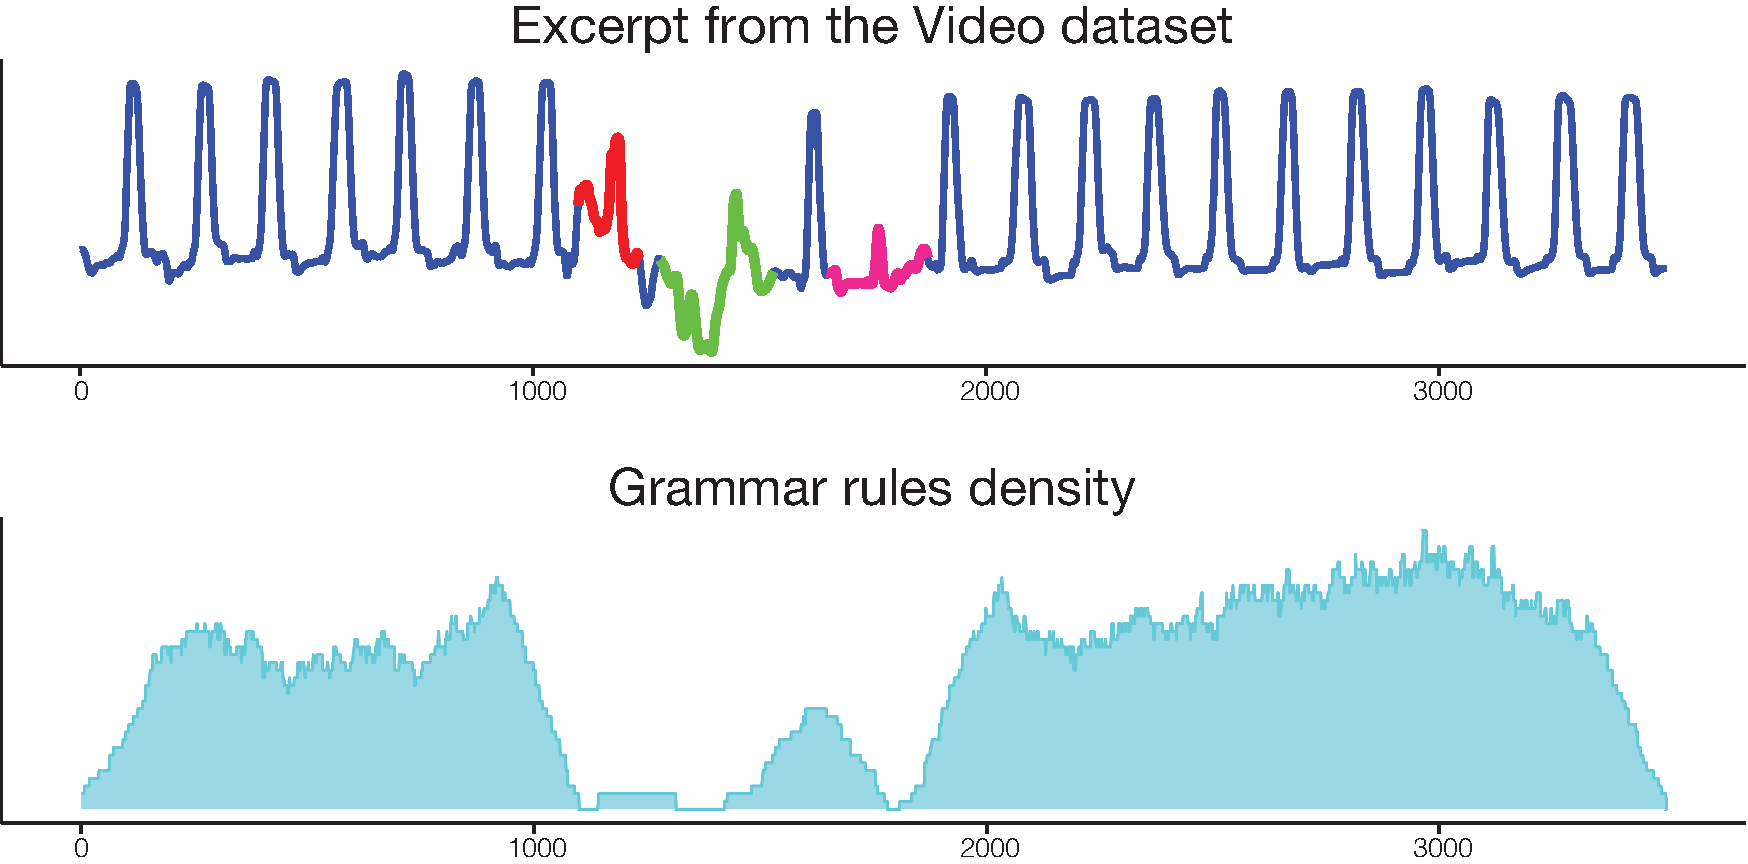
\includegraphics[width=84mm]{ECG13.pdf}
  \caption{An example of multiple anomalous events found in a recorded video time series \cite{param_free} shown at the top panel. The \textit{rule density curve}, which we propose in this paper, and which is built in linear time and space, is shown in the bottom panel. Reflecting the hierarchical grammar structure, the rule density curve reaches its minima where no algorithmic redundancy is observed, pinpointing anomalous locations precisely.}
  \label{fig:video1}
\end{figure}
\textbf{Z-normalization} is a process that brings the mean of a subsequence $C$ to zero and its standard deviation to one.

Given two time series subsequences $C$ and $M$, both of length $n$, the distance between them is a real number that accounts for how much these subsequences are different, and the function which outputs this number when given $C$ and $M$ is called the \textbf{distance function} and denoted $Dist(C,M)$. One of the most commonly used distance functions is the \textbf{Euclidean distance}, which is the square root of the sum of the squared differences between each pair of the corresponding data points in $C$ and $M$.

One of our proposed techniques is built upon determining if a given subsequence $C$ is similar to other subsequences $M$ under distance measure $Dist$. This notion is formalized in the definition of a match:

\textbf{Match}: Given a positive real number $t$ (i.e., threshold) and subsequences $C$ and $M$, if $Dist(C,M)\leq t$ then subsequence $M$ is a match to $C$.

When searching for potential anomalies using a distance function, it is important to exclude self matches, which are subsequences that overlap the subsequence currently being considered. Such self-matches can yield degenerate and unintuitive solutions as discussed in \cite{hot_sax}. For two subsequences $C$ and $M$ we define a non-self match:

\textbf{Non-self match}: Given a subsequence $C$ of  length $n$ starting at position $p$ of time series $T$, the subsequence $M$ beginning at $q$ is a non-self match to $C$ at distance $Dist(C,M)$ if $|p-q| \geq n$.

As mentioned, one of the most effective methods for time series anomaly detection is via discord discovery. Formally, it is defined as:

\textbf{Time Series Discord}: Given a time series $T$, the time series subsequence $C \in T$ is called the discord if it has the largest Euclidean distance to its nearest non-self match \cite{hot_sax}. Thus, time series discord is a subsequence within a time series that is maximally different to all the rest of subsequences in the time series, and therefore naturaly captures the most unusual subsequence within the time series \cite{hot_sax}.

\subsection{Problem definition}
The task of finding a structural time series anomaly is defined as 

\textit{Given a time series $T$, find a subsequence $C$ that is the most (structurally) different from the rest of the observed subsequences}.

This task, however, is very difficult to solve in its general form without a notion of the context   \cite{chan_anomaly}.  The context is information that can be induced from the structure of the dataset or specified as a part of the problem. It places constraints on both the search space and the results, making it possible to find a meaningful solution. Based on this rationale, we re-define the anomaly discovery problem as: 

\textit{Given a time series $T$ and some context, find a subsequence $C$ that is the most structurally different from others and which can be related to the context}.

In discords---the current state of the art in structural anomaly detection \cite{chan_anomaly}---the context is provided by the user-defined anomaly length, and the notion of the ``most structurally different'' is defined as the largest Euclidean distance to the nearest non-self match. Both constraints, while defining the problem and the solution exactly, place severe restrictions on the result by assuming unrealistic a priori knowledge about the exact anomaly length. 

In this work we address this issue by allowing the discord length to vary in boundaries that are consistent with the time series context. Toward this end, we represent the context as a hierarchical grammar structure obtained through the processes of time series symbolic discretization and context-free grammar induction. In turn, by exploiting the use frequencies of the induced grammar rules, our technique finds the most unusual rules which we consider as discord candidates to be evaluated and which, naturally, vary in length.

\section{Grammar-Based Time Series Decomposition}\label{discretization}
Before describing our approach in detail, consider the following example showing the context-free grammar properties used in our approach. Let 
\begin{center}
\vspace{-1mm}
%$S$ = $a\,b\,c\ \ a\,b\,c\ \ c\,b\,a\ \ XXX\, \ a\,b\,c\ \  a\,b\,c\ \ c\,b\,a$
$S$ = $abc\ \ abc\ \ cba\ \ xxx\ \ abc\ \ abc\ \ cba$

\vspace{-1mm}
\end{center}
be the input string under analysis (e.g. derived from a time series and reflecting its structure). For reason that will become clearer later, the input string consists of a sequence of \textit{words} (in this example, 3-letter words or triplets). Each triplet is considered an atomic unit, or a \textit{terminal} in the sequence. The task is to compress this input sequence by grammar induction.

A careful look at the string shows that there are repeated patterns \textit{abc\;abc\;cba} separated by \textit{xxx}. Ideally, we expect the grammar induction or compression algorithm to reflect this, as shown in the possible grammar for input $S$:
\begin{table}[!h] 
%\caption{A possible grammar for the input string $S$}
\centering
\begin{tabularx}{\linewidth}{sb} % centered columns (2 columns) 
\hline
Grammar Rule & Expanded Grammar Rule \\ 
\hline 
R0 $\rightarrow$ R1 xxx R1 & \textcolor{red}{abc abc} \textcolor{cyan}{cba} \textcolor{blue}{xxx} \textcolor{red}{abc abc} \textcolor{cyan}{cba} \\ 
R1 $\rightarrow$ R2 \textcolor{cyan}{cba} & \textcolor{red}{abc abc} \textcolor{cyan}{cba}\\
R2 $\rightarrow$ \textcolor{red}{abc abc} & \textcolor{red}{abc abc} \\
\hline
\end{tabularx} 
\label{table:rules} % is used to refer this table in the text 
\end{table} 

As shown, the grammar induction algorithm has reduced the length of the input string (i.e., compressed it) by creating a grammar whose rules are encoded by \textit{non-terminals} $R1$ and $R2$, which reveal repeated patterns in the input. 

In previous work, we have shown that by the analysis of a grammar built upon time series discretization it is possible to identify recurrent patterns, i.e. time series motifs \cite{grammarviz}. Since anomaly detection can be viewed as the inverse problem to motif discovery, in this work, we argue that symbols that are rarely used in grammar rules (i.e. \textit{\textcolor{blue}{xxx}}) may aid in anomaly detection as well.  The intuition is that subsequences of any length that never or rarely occur in grammar rules are non-repetitive and are thus most likely to be unusual or anomalous.

To illustrate this, suppose we annotate each word of the input string $S$ with the number of rules that the word appears in excluding the top-level rule R0. The input string $S$ becomes the following:
\begin{center}
%$S = a_{2}b_{2}c_{2}\ a_{2}b_{2}c_{2}\ c_{1}b_{1}a_{1}\ X_{0}X_{0}X_{0}\ a_{2}b_{2}c_{2}\ a_{2}b_{2}c_{2}\ c_{1}b_{1}a_{1}$

$S = abc_{2}\ abc_{2}\ cba_{1}\ xxx_{0}\ abc_{2}\ abc_{2}\ cba_{1}$
\end{center}

All occurrences of the word $abc$ have a count of 2 because they appear in both $R1$ and $R2$; the word $cba$ has count of 1 since it appears only in $R1$; whereas the word $xxx$ has a count 0, because it is not a part of any rule. Since the counts naturally reflect the algorithmic compressibility of the sequence of terminal and non-terminal symbols, the triplet $xxx_{0}$ is algorithmically incompressible by the grammar induction algorithm and thus algorithmically random. In turn, if the input string $S$ is derived by discretizing a time series into a sequence of words, where each word corresponds to a time series subsequence, then based on our hypothesis, the subsequence in the time series that $xxx$ represents is a potential anomaly.

Note that when identifying a potential anomaly we have not used any explicit distance computation between terminal or non-terminal symbols, grammar rules, or their corresponding (i.e., raw) subsequences. Moreover, note that the time series discretization technique SAX \cite{sax} and the grammatical inference algorithm Sequitur \cite{sequitur} that we rely upon, also do not compute any distance (i.e., they do not explicitly measure how far apart objects are). Hence, unlike most anomaly discovery algorithms, our approach does not require any distance computation to discover and to rank multiple potential anomalies. 

Discovered in the above example potential anomaly is the most unusual substring of a larger input string in terms of the grammatical inference algorithm of choice. Specifically, in contrast to other terminal symbols, the word $xxx$ is not included in any of grammatical rules -- the property that is discovered and accounted for by the grammatical inference algorithm. Thus, the discovered anomalous substring is analogous in meaning to a \textit{time series discord}. However, our approach determines the anomalous subsequence length automatically in the course of grammar induction process, whereas the discord discovery algorithm requires the length of a potential anomaly to be known in advance. 

Based on the intuition shown above, we shall present two algorithms that enable the discovery of variable-length anomalies. Before that, we discuss time series discretization and grammatical inference -- the procedures upon which our techniques are built.

\subsection{Discretization} 
Since grammar induction algorithms are designed for discrete data, we begin by discretizing a continuous time series with SAX (Symbolic Aggregate approXimation) \cite{sax}. In addition, since an anomaly is a local phenomenon,  we apply SAX to subsequences extracted via a sliding window. SAX performs discretization by dividing \textit{z}-normalized subsequence into $w$ equal-sized segments. For each segment, it computes a mean value and maps it to symbols according to a pre-defined set of breakpoints dividing the distribution space into $\alpha$ equiprobable regions, where $\alpha$ is the alphabet size specified by the user. This \textit{subsequence discretization} process \cite{lin_motifs} outputs an ordered set of SAX words, where each word corresponds to the leftmost point of the sliding window, and which we process with numerosity reduction at the next step.

As an example, consider the sequence $S1$ where each word (e.g. $aac$) represents a subsequence extracted from the original time series via a sliding window and discretized with SAX (the subscript following each word denotes the starting position of the corresponding subsequence in the time series):

%\footnote{Note that in the prior motivating example shown in Section \ref{discretization}, for simplicity and to convey the idea, each symbol was considered as a terminal symbol, whereas in our SAX-based discretization process, each SAX word is treated as an atomic, terminal symbol.}:
\begin{center} 
$S1= aac_{1}\, aac_{2}\, abc_{3}\, abb_{4}\, acd_{5}\, aac_{6}\, aac_{7}\, aac_{8}\, abc_{9}\, \dots$
\end{center}

In contrast to many SAX-based anomaly discovery techniques that store SAX words in a trie or a hash table for optimizing the search, and essentially throw away the ordering information, we argue that the sequential ordering of SAX words provides valuable \textit{contextual information}, and is the key for allowing variable-length pattern discovery. 

\subsection{Numerosity reduction} As we have shown in \cite{lin_motifs}, neighboring subsequences extracted via sliding window are often similar to each other. When combined with the smoothing properties of SAX, this phenomenon persists through the discretization, resulting in a large number of consecutive SAX words that are identical. Later, these yield a large number of trivial matches significantly affecting performance. To address this issue, we employ a numerosity reduction strategy: if in the course of discretization, the same SAX word occurs more than once consecutively, instead of placing every instance into the resulting string, we record only its first occurrence. Applied to $S1$, this process yields:
\begin{center}
 $S1 = \textit{aac}_{1}~ \textit{abc}_{3}~ \textit{abb}_{4}~ \textit{acd}_{5}~ \textit{aac}_{6}~ \textit{abc}_{9}$ 
\end{center}
In addition to speeding up the algorithm and reducing its space requirements, the numerosity reduction procedure provides an important feature in this work -- it naturally enables the discovery of variable-length anomalies as we show next. 

\subsection{Grammar induction on SAX words}\label{rule_utility}
Next, the reduced (from repetitions) sequence of SAX words is inputted into Sequitur \cite{sequitur}, our grammar induction algorithm of choice, to build a context-free grammar. 

Sequitur is a linear time and space algorithm that derives the context-free grammar from a string incrementally. Processing the input string from left to right, Sequitur builds the hierarchical structure of a context-free grammar by identifying and exploiting symbol correlations while maintaining the two constraints of uniqueness and utility at all times. Although simple in design, Sequitur has been shown to be competitive with state of the art compression algorithms -- the property which allows us to use the notion of Kolmogorov complexity. In addition, Sequitur performance tends to improve with the growth of the input string size \cite{compression}. 

When applied to a sequence of SAX words, Sequitur treats each word as an input string token and builds the context-free grammar's hierarchical structure. This structure recursively reduces all \textit{digrams} that are consecutive pairs of tokens (terminal or non-terminal) occurring more than once in the input string to a single new non-terminal symbol. 

To reiterate the benefit of the numerosity reduction strategy and how it lends itself to variable-length pattern discovery with Sequitur, consider the single grammar rule $R1$ generated by Sequitur from the string \textit{S1} as shown here:

\begin{table}[h] 
\centering
\begin{tabularx}{\linewidth}{db}
\hline
Grammar Rule & Expanded Grammar Rule \\
\hline
$\text{R0}~ \rightarrow~ \text{R1}~ \text{abb}~ \text{acd}~ \text{R1}$ & $ \textcolor{red}{aac}_{1}~ \textcolor{red}{abc}_{3}~ abb_{4}~ acd_{5}~ \textcolor{red}{aac}_{6}~ \textcolor{red}{abc}_{9}$ \\ 
$\text{R1}~ \rightarrow~ \text{aac}~ \text{abc} $ & $\textcolor{red}{aac}~ \textcolor{red}{abc}$ \\
\hline
\end{tabularx}
\label{table:rulesS1} % is used to refer this table in the text 
\end{table} 

In this grammar, $R1$ concurrently maps to substrings of different lengths: $S1_{[1:3]}$ of length 3 (i.e., $aac_{1}\, aac_{2}\, abc_{3}$) and $S1_{[6:9]}$ of length 4 (i.e., $aac_{6}\, aac_{7}\, aac_{8}\, abc_{9}$), respectively. The potential anomalous substring ``$abb_{4}\,acd_{5}$'' has length 2. Since each SAX word corresponds to a \textit{single point} of the input time series (a subsequence starting point), $R1$ maps to its subsequences of variable lengths. 

\subsection{Mapping rules to subsequences}
As shown in the above example, by keeping SAX words' offsets throughout the procedures of discretization and grammar induction, our algorithm is able to map rules and SAX words back to their original time series subsequences. 

\subsection{Pattern mining with Sequitur}
Previously in \cite{grammarviz}, we proposed GrammarViz, an algorithm for variable-length time series motif discovery that makes full use of the hierarchy in Sequitur's grammar. We showed the ability of the proposed algorithm to discover recurrent patterns of variable lengths.  This is due to several properties of the algorithm, including: the data smoothing capability of SAX, numerosity reduction which enables the patterns' variable length, and Sequitur's \textit{utility} constraint which ensures that all of the grammar's non-terminals correspond to recurrent patterns. We later implemented visualization software based on this concept \cite{grammarviz2} that also provides a pilot module demonstrating the potential for a grammar-based approach to identify anomalies. 

In this work, we formally introduce the notion of the \textit{rule density curve} which is the key to our grammar-driven anomaly detection algorithm. Simply put, the rule density curve reflects the number of Sequitur grammar rules that span a time series point. We also provide theoretical background for our empirical observations. For this, we emphasize the role of the second Sequitur constraint, \textit{digram uniqueness}, which ensures that none of the digrams processed by the algorithm (i.e., compressed into non-terminals) repeats itself.  This property guarantees the \textit{exhaustiveness of the search} for algorithmically exploitable redundancies in the input string, and consequently \textit{asymptotically maximal compression} of the output string \cite{compression}. Both properties allow us to put our approach within the Kolmogorov complexity framework based on the  algorithmic compressibility and relate algorithmically incompressible subsequences to anomalies as we discuss in the next section.

\section{Grammar-driven Anomaly\\ Discovery}\label{algorithms}
Within Kolmogorov complexity research, it has been proven that \textit{algorithmic incompressibility is a necessary and sufficient condition for randomness} \cite{grigorieff, li_vitanyi}, thanks to the elegant statistically-sound theory developed by Martin-L\"{o}f \cite{per_lof}. This theoretically grounds our intuition and effectively supports the claim that if a grammar induction algorithm is incapable of encoding a subsequence by finding exploitable correlations within the input string, such a subsequence is random within the context of the input string and applied algorithm. We call such subsequences \textit{algorithmically anomalous} and equate them to time series anomalies.  

Let us explain the utility of ``algorithmic anomalousness''. When searching for an anomaly in a time series, we expect that while the true generative process is unknown, it is likely to be regular and that the time series reflects these regularities. At the same time, we also assume that the time series may contain some abnormal segments, whose identification is our goal. Further, assuming that the discretization process preserves these regularities and irregularities, the Sequitur algorithm should be able to learn the regularities and effectively compress the input string. However, due to its invariants of utility and uniqueness, Sequitur will not be able to form rules that contain symbolic subsequences occurring just once in the input string, because it will not be able to find any short- or long-term correlations between them and the rest of the string -- the property that reflects irregularity and defines a variable-length anomaly in the most natural way. 

Based on the intuition behind algorithmic anomalousness we propose two algorithms for grammatical compression-driven variable-length anomaly discovery from time series. Configured only by the discretization parameters, both algorithms are capable of efficient discovery of putative anomalous subsequences without any prior knowledge of their length, shape, or minimal occurrence frequency. While the result produced by the first algorithm is an approximate solution, our second algorithm is based on explicit distance computations and outputs time series discords of variable length.

\begin{figure}[t]
  \centering
  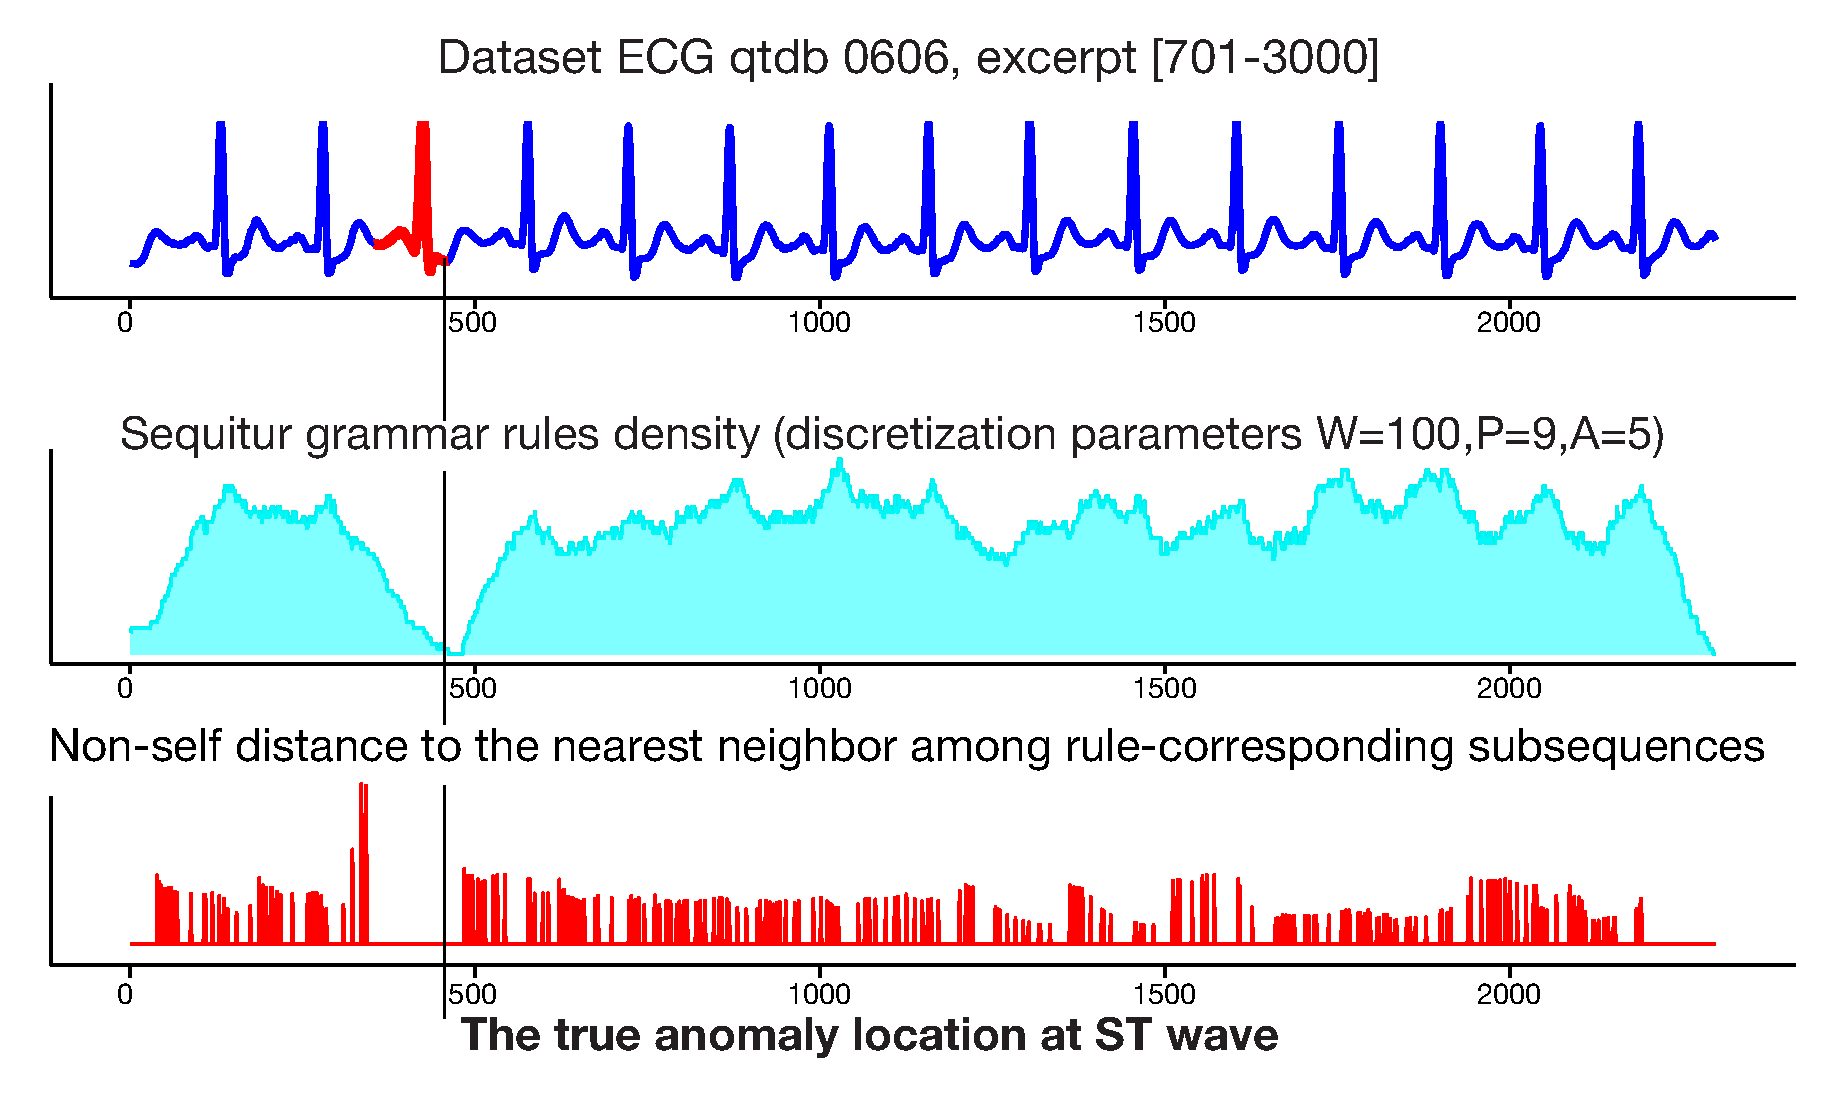
\includegraphics[width=84mm]{Figure1_ECG0606.pdf}
  \caption{Anomaly discovery in ECG dataset. Top panel shows the anomalous heartbeat location. Middle panel shows that the rule density curve clearly identifies the true anomaly by its global minimum. Bottom panel confirms that the RRA-reported discord has indeed the largest distance to its nearest non-self match.}
  \label{fig:ecg}
\end{figure}

\subsection{Efficient, rule density-based anomaly\\ discovery}\label{density_curve}
To efficiently discover approximate anomalies, we propose to compute the rule density curve for the input time series. Toward that end, an empty array of length $m$ (the length of the time series), is first created. Each element in this array corresponds to a time series point and is used to keep count of the grammar rules that span (or ``cover'') the point. Second, since the locations of corresponding subsequences for all grammar rules are known, by iterating over all grammar rules the algorithm increments a counter for each of the time series points that the rule spans. After this process each element of the array contains a value indicating the total number of grammar rules that covers the corresponding time series point. The curve that corresponds to the array's values is the \textit{rule density curve}. As an example, consider the rule density curves shown in the middle panels of Figures \ref{fig:ecg} and \ref{fig:dutch_PD}.

Since each SAX string corresponds to a subsequence starting at some position of the time series, the points whose rule density counters are global minima correspond to the grammar symbols (terminals or non-terminals) whose inclusion in the grammar rules are minimal. These subsequences are algorithmically anomalous by our definition and we argue that the \textit{rule density curve intervals that contain minimal values correspond to time series anomalies}, and our algorithm simply outputs these intervals.

Consider the example shown in Figure \ref{fig:ecg}. The top panel shows an excerpt of an ECG time series with a highlighted instance of an anomalous heartbeat featuring a very subtle premature ventricular contraction. The middle panel shows a significant drop in the grammar rule density over the interval 462-484, which is in perfect alignment with the ground truth -- an expert's annotation of an anomaly occuring in the ST interval of the ECG curve (as discussed in \cite{hot_sax}). Similar to that, the global minima of the rule density curve shown in the middle panel of Figure \ref{fig:dutch_PD} pinpoints the weekly interval that has the most unusual power consumption pattern (the dataset in the top panel of Figure \ref{fig:dutch_PD} shows the power consumption history of a Dutch research facility for the entire year of 1997 \cite{dutchpd}).

The rule density-based approach is capable of discovering multiple anomalies of variable length.  When given a fixed threshold, it simply reports contiguous points of the input time series whose density is less than the threshold value. If needed, an additional ranking criterion can be defined, such as a minimal anomaly length or a statistically sound criterion based on probabilities.

Note that even though we need to specify the sliding window length, it is only the initial ``seed'' value. Unlike most existing algorithms in which this subsequence length is the exact length of the anomaly, anomalies reported by our technique are not bounded by the seed length and may range from very short to very long time spans.

\begin{figure}[t]
 \centering
 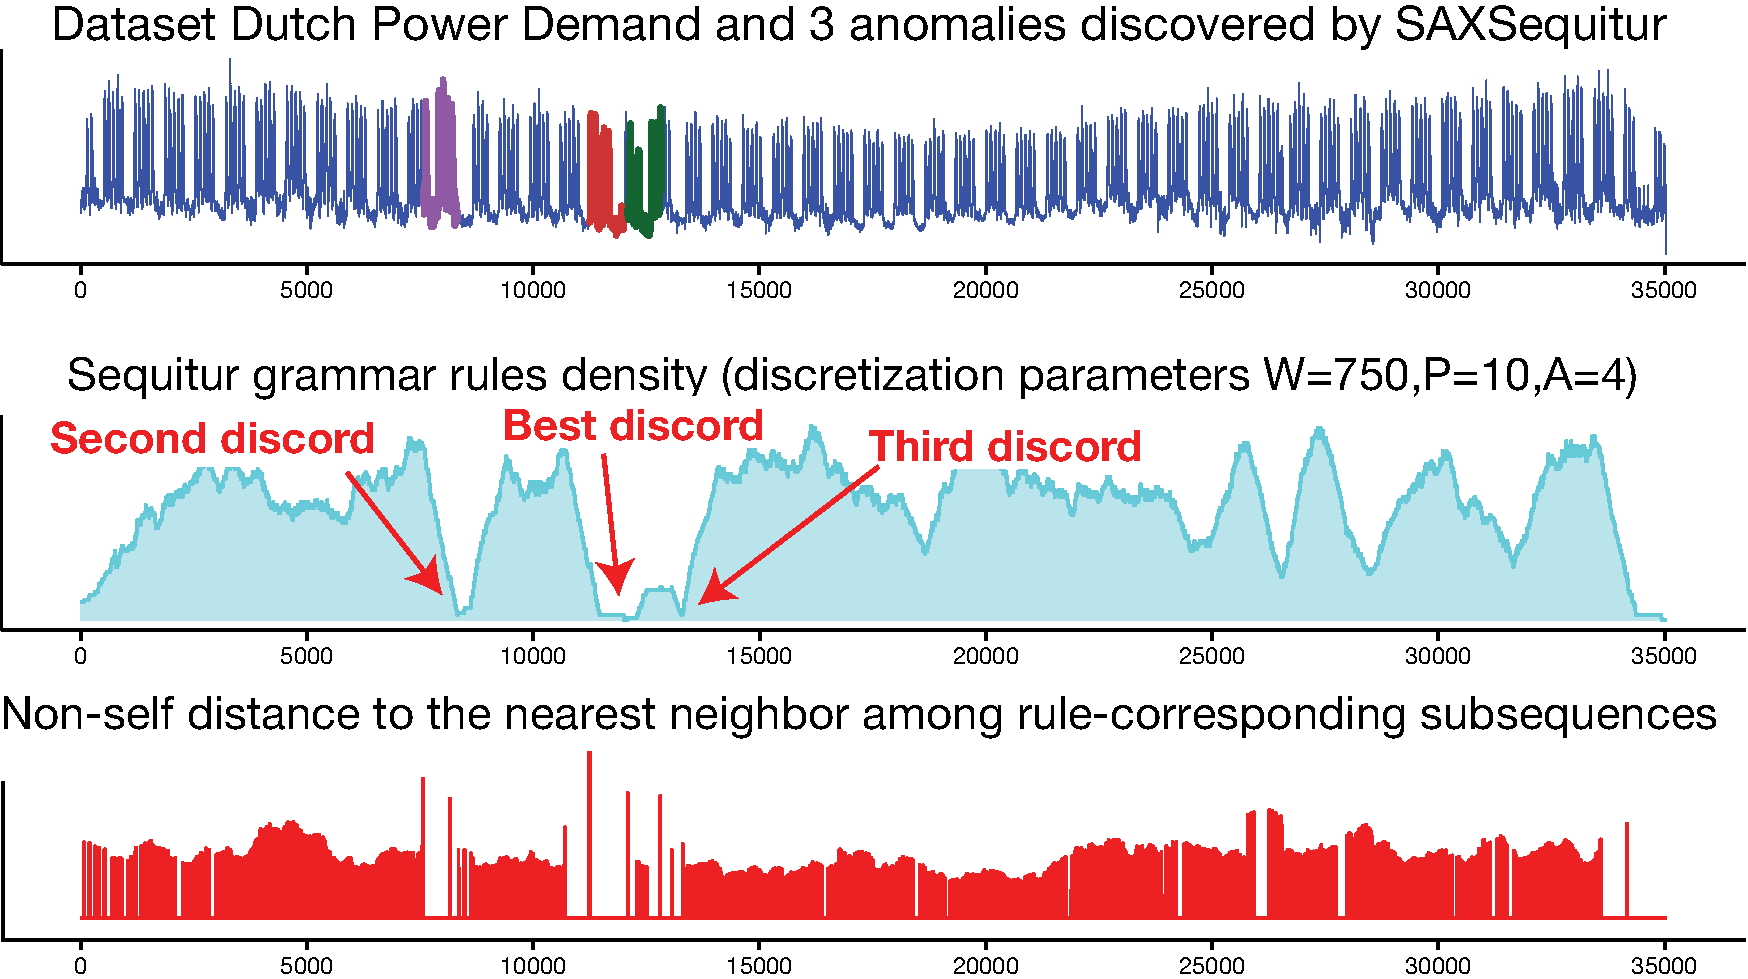
\includegraphics[width=84mm]{DutchPD_new.pdf}
 \caption{Multiple discord discovery in Dutch power demand data \cite{dutchpd}. Top panel shows 52 weeks of power demand by a research facility. Middle panel shows that while the rule density-based technique was able to discover the best discord, others are difficult to discriminate. The bottom panel shows distances to the nearest non-self match computed for each rule-corresponding subsequence, which allows for the ranking of discords discovered with RRA.}
 \vspace{2em}
 \label{fig:dutch_PD}
 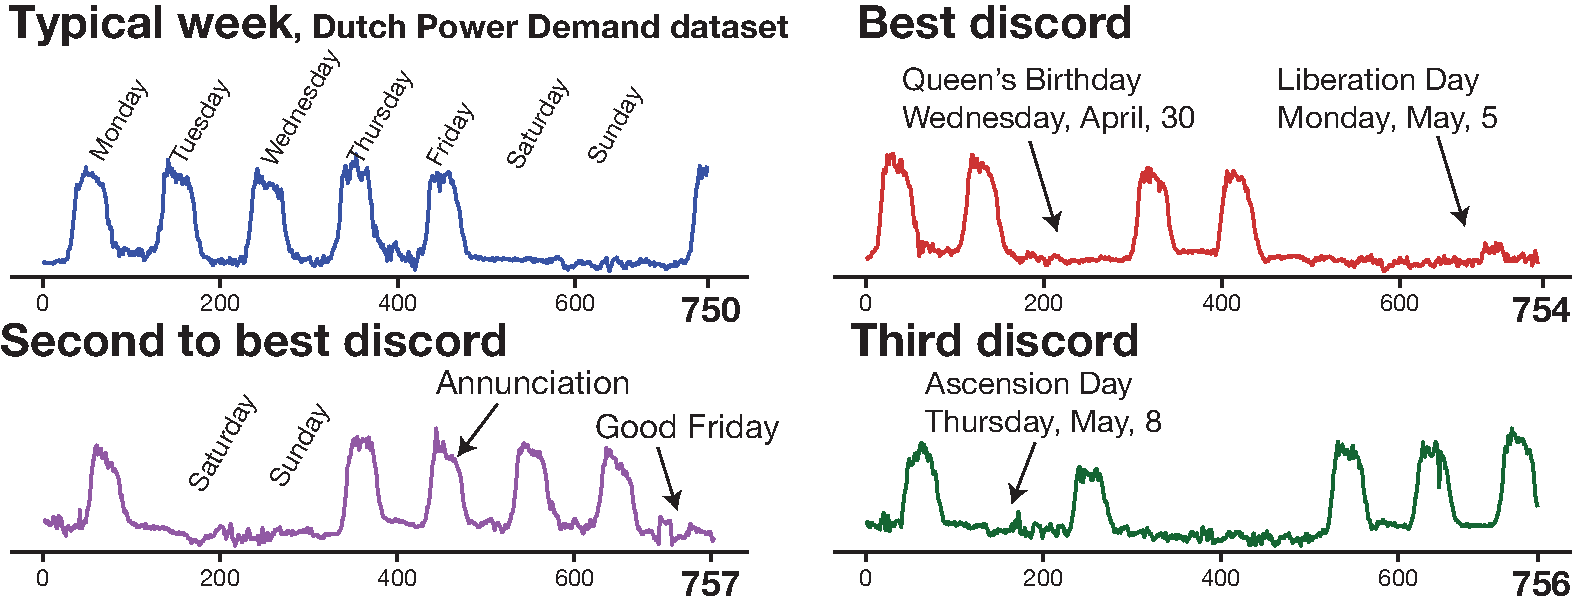
\includegraphics[width=84mm]{DutchPD_new1.pdf}
 \caption{A detailed view of RRA-ranked variable length discords discovered in the Dutch power demand dataset. All of them highlight time intervals where typical weekly patterns are interrupted by state holidays.}
 \label{fig:dutch_PD2}
\end{figure}

Another distinguishable and desirable characteristic of this approach is its efficiency. It has linear time and space complexity since the sequential processing of SAX, Sequitur, and the global minima search take linear time and space. This efficiency, when combined with effective rule density curve-based visualization, enables the user to interactively explore the dataset and to refine discretization parameters and the anomaly selection threshold.

\subsection{Exact, distance-based anomaly discovery}
If the time series under analysis has low regularity (an issue that impacts the grammar's hierarchy) or the discretization parameters are far from optimal and regularities are not conveyed into the discretized space, the rule density-based anomaly discovery technique may fail to output true anomalies. In addition, some applications may require additional anomaly evidence or  ranking. To address this, we propose a second variant of a grammar-driven variable-length anomaly discovery algorithm based on an explicit distance computation which outputs discords -- the subsequences whose distance to their nearest non-self match is the largest. Since anomalous subsequences correspond to rare grammar rules, we call the algorithm RRA (Rare Rule Anomaly).

\noindent\begin{minipage}{82mm}
\begin{algorithm}[H]
\small
\caption{RRA algorithm}\label{algorithm2}
\begin{algorithmic}[1]
\Function{Find\_discord}{$T,Intervals,Outer,Inner$}
 \State $\text{best\_so\_far\_dist} = 0 $
 \State $\text{best\_so\_far\_loc} = \text{NaN} $
 \For{\textbf{each} $p$ in $Intervals$ ordered by $Outer$}
 %\Comment{We completely}
 %\Statex{}\Comment{change this heuristic}
    \State nearest\_neighbor\_dist = Infinity
    \For{\textbf{each} $q$ in $Intervals$ ordered by $Inner$}
    %t_{p},...,t_{p+n-1}, t_{q},...,t_{q+n-1})$}
    %\Comment{We partially change}
    %\Statex{}\Comment{this heuristic}
       \If {$| p_{0} -– q_{0} | \geq \; Length(p)\ ^{1}$ } 
           \State {current\_dist $=Dist(p,q)$}
           \If { current\_dist $<$ best\_so\_far\_dist}
               \State {\textbf{break}} 
           \EndIf 
           \If {current\_dist $<$ nearest\_neighbor\_dist }
               \State {nearest\_neighbor\_dist = current\_dist}
           \EndIf 
       \EndIf 
       \If {nearest\_neighbor\_dist $>$ best\_so\_far\_dist} 
           \State {best\_so\_far\_dist = nearest\_neighbor\_dist} 
           \State {best\_so\_far\_loc = p}
       \EndIf          
    \EndFor
 \EndFor
 \State \textbf{return} $(\text{best\_so\_far\_dist}, \text{best\_so\_far\_loc})$
\EndFunction
\end{algorithmic}
\end{algorithm}
\vspace{-1em}
\footnotemark[1]{$p_{0}$ and $q_{0}$ are the global indexes (in $T$) of the first points of subsequences $p$ and $q$ respectively. In this line we check that currently analyzed subsequences do not overlap (i.e., $q$ is non-self match of $p$).}
\vspace{2em}
\end{minipage}

The RRA algorithm is based on the HOTSAX framework initially proposed in \cite{hot_sax} for the discord discovery. The algorithm's input includes the original time series $T$, a list of variable length subsequences corresponding to grammar rules which we call $Intervals$, and two heuristics: $Inner$ and $Outer$, which can be applied to list of subsequences. 

Similar to HOTSAX, our algorithm iterates over all candidate subsequences in the outer loop (line 4 of Algorithm \ref{algorithm2}) while computing distances to all other non-self matches in the inner loop (lines 6--8; $p_{0}$ and $q_{0}$ in line 7 are the indexes) and selecting the closest non-self match (lines 9--15). The candidate subsequence from the outer loop which yields the largest distance to a non-self match is output as the result. In HOTSAX, the candidates in the outer ($Outer$) and inner ($Inner$) loops are ordered based on the SAX representations of the candidate subsequences such that the order of consideration is as close to the \textit{optimal} ordering (i.e., the ordering that would result in the most elimination of computations) as possible. However, as mentioned earlier, HOTSAX candidates are restricted by their subsequence length. Our proposed technique differs from HOTSAX in that subsequences (i.e., $Intervals$ in Algorithm \ref{algorithm2}) and their ordering for the inner ($Inner$) and outer ($Outer$) loops are provided as the input based on the information derived from grammar.

Specifically, $Intervals$ subsequences are those that correspond to the grammar rules plus all continuous subsequences of the discretized time series that do not form any rule. The $Outer$ subsequence ordering utilizes the information derived from a hierarchical grammar structure -- we order subsequences in  ascending order of their corresponding rule usage frequency (note that continuous subsequences of the discretized time series that do not form any rule have frequency 0 and are thus considered first). The intuition  behind this ordering is simple and is a reflection of the previously discussed properties of algorithmically anomalous subsequences. That is, the sooner we encounter the \textit{true} anomaly, the larger the $best\_so\_far\_dist$ is, and the more computations we can potentially eliminate later on (line 9). 

\begin{table*}[ht]
\caption{Performance comparison for brute-force, state-of-the-art, and the proposed exact discord discovery algorithms.}
\label{perf_table}
\centering
\begin{small}
\begin{tabularx}{\linewidth}{X r r r r r r r r}
\toprule
\parnoteclear
Dataset name and discretization & Length & \multicolumn{3}{c}{Number of calls to the distance function} & Reduction in & \multicolumn{3}{r}{\textit{HOTSAX} \& \textit{RRA} dis-} \\ 
 \cline{3-5}
param. (window, PAA, alphabet) &  & Brute-force & \textit{HOTSAX}
& \textit{RRA} & distance calls & \multicolumn{3}{r}{cords length and overlap}\\
\midrule
\raggedright
Daily commute (350,15,4) & 17'175 & 271'442'101 & 879'067 & 112'405 & 87.2\% & \qquad& 350 / 366 & 100.0\%\\
Dutch power demand (750,6,3) & 35'040 & $1.13 \times 10^{9}$ & 6'196'356 & 327'950 & 95.7\% & & 750 / 773 & 96.3\%\\
ECG 0606 (120,4,4) & 2'300 & 4'241'541 & 72'390 & 16'717 & 76.9\%& & 120 / 127 & 79.2\% \\
ECG 308 (300,4,4) & 5'400 & 23'044'801 & 327'454 & 14'655 & 95.5\%& & 300 / 317 & 97.7\% \\
ECG 15 (300,4,4) & 15'000 & 207'374'401 & 1'434'665 & 111'348 & 92.2\%& & 300 / 306 & 65.0 \%\\
ECG 108 (300,4,4) & 21'600 & 441'021'001 & 6'041'145 & 150'184 & 97.5\%& & 300 / 324 & 89.7\%\\
ECG 300 (300,4,4) \parnote{{\small RRA reported the best discord discovered with HOTSAX as the second discord (Figure \ref{fig:ecg300}).}} & 536'976 & $288 \times 10^{9}$ & 101'427'254 & 17'712'845 & 82.6\%& & 300 / 312 & 83.0\% \\
ECG 318 (300,4,4) & 586'086 & $343 \times 10^{9}$ & 45'513'790 & 10'000'632 & 78.0\%& & 300 / 312 & 80.7\% \\
Respiration, NPRS 43 (128,5,4) & 4'000 & 14'021'281 & 89'570 & 45'352 & 49.3\%& & 128 / 135 & 96.0\% \\
Respiration, NPRS 44 (128,5,4) & 24'125 & 569'753'031 & 1'146'145 & 257'529 & 77.5\%& & 128 / 141 & 61.7\% \\
Video dataset (gun) (150,5,3) & 11'251 & 119'935'353 & 758'456 & 69'910 & 90.8\%& & 150 / 163 & 89.3\% \\
Shuttle telemetry, TEK14 (128,4,4) & 5'000 & 22'510'281 & 691'194 & 48'226 & 93.0\%& & 128 / 161 & 72.7\%\\
Shuttle telemetry, TEK16 (128,4,4) & 5'000 & 22'491'306 & 61'682 & 15'573 & 74.8\%& & 128 / 138 & 65.6\%\\
Shuttle telemetry, TEK17 (128,4,4) & 5'000 & 22'491'306 & 164'225 & 78'211 & 52.4\%& & 128 / 148 & 100.0\%\\
\bottomrule
\end{tabularx}
\raggedright
\parnotes
\end{small}
\end{table*}

The $Inner$ candidate match ordering is also based on grammar information. First, having a candidate subsequence from a grammar rule selected in the $Outer$ loop, we consider all other subsequences from the same rule as possible nearest non-self matches. After this step, the rest of the subsequences are visited in  random order. The intuition behind this ordering is also simple -- the subsequences corresponding to the same Sequitur rule are very likely to be highly similar. Thus, considering those in the beginning of $Inner$ loop allows us to potentially encounter a distance that is smaller than $best\_so\_far\_dist$ sooner and to benefit from early abandoning (lines 9--10 of the Algorithm \ref{algorithm2}) while considering all other candidates in the $Outer$ loop. Since RRA operates with rule-corresponding subsequences of variable lengths, when searching for nearest non-self match we employ the Euclidean distance normalized by the subsequence length, which favors shorter subsequences for the same distance value: 

\begin{equation}
  Dist(p,q) = \frac{\sqrt{\sum_{i=1}^n (p_i-q_i)^2}}{Length(p)} \label{dist}
\end{equation}
%\vspace{0.2em}
When run iteratively, excluding the current best discord from $Intervals$ list, RRA outputs a ranked list of multiple co-existing discords of variable length, as shown in Figures \ref{fig:dutch_PD} and \ref{fig:dutch_PD2}. The bottom panels of Figures \ref{fig:ecg} and \ref{fig:dutch_PD} indicate locations and true distances from each time series subsequence corresponding to a grammar rule to its nearest non-self match by a vertical line placed at the rule beginning and whose height equals the distance.
\vspace{1em}
\section{Experimental Evaluation}\label{evaluation}
We evaluated both proposed techniques on a number of datasets previously studied in \cite{hot_sax} that include Space Shuttle Marotta Valve telemetry (TEK), surveillance (Video data\-set), health care (electrocardiogram and respiration change), and industry (Dutch Power Demand).  We also evaluated on a new dataset of spatial trajectories.  We compared the performance of the proposed algorithms against brute force and HOTSAX \cite{hot_sax} discord discovery algorithms. Since RRA returns discords of variable length that may differ significantly from the specified sliding window length, we show the RRA discord recall rate as the overlap between discords discovered by HOTSAX and RRA algorithms in the last column of Table \ref{perf_table}. 

\begin{figure}[t]   
   \centering
   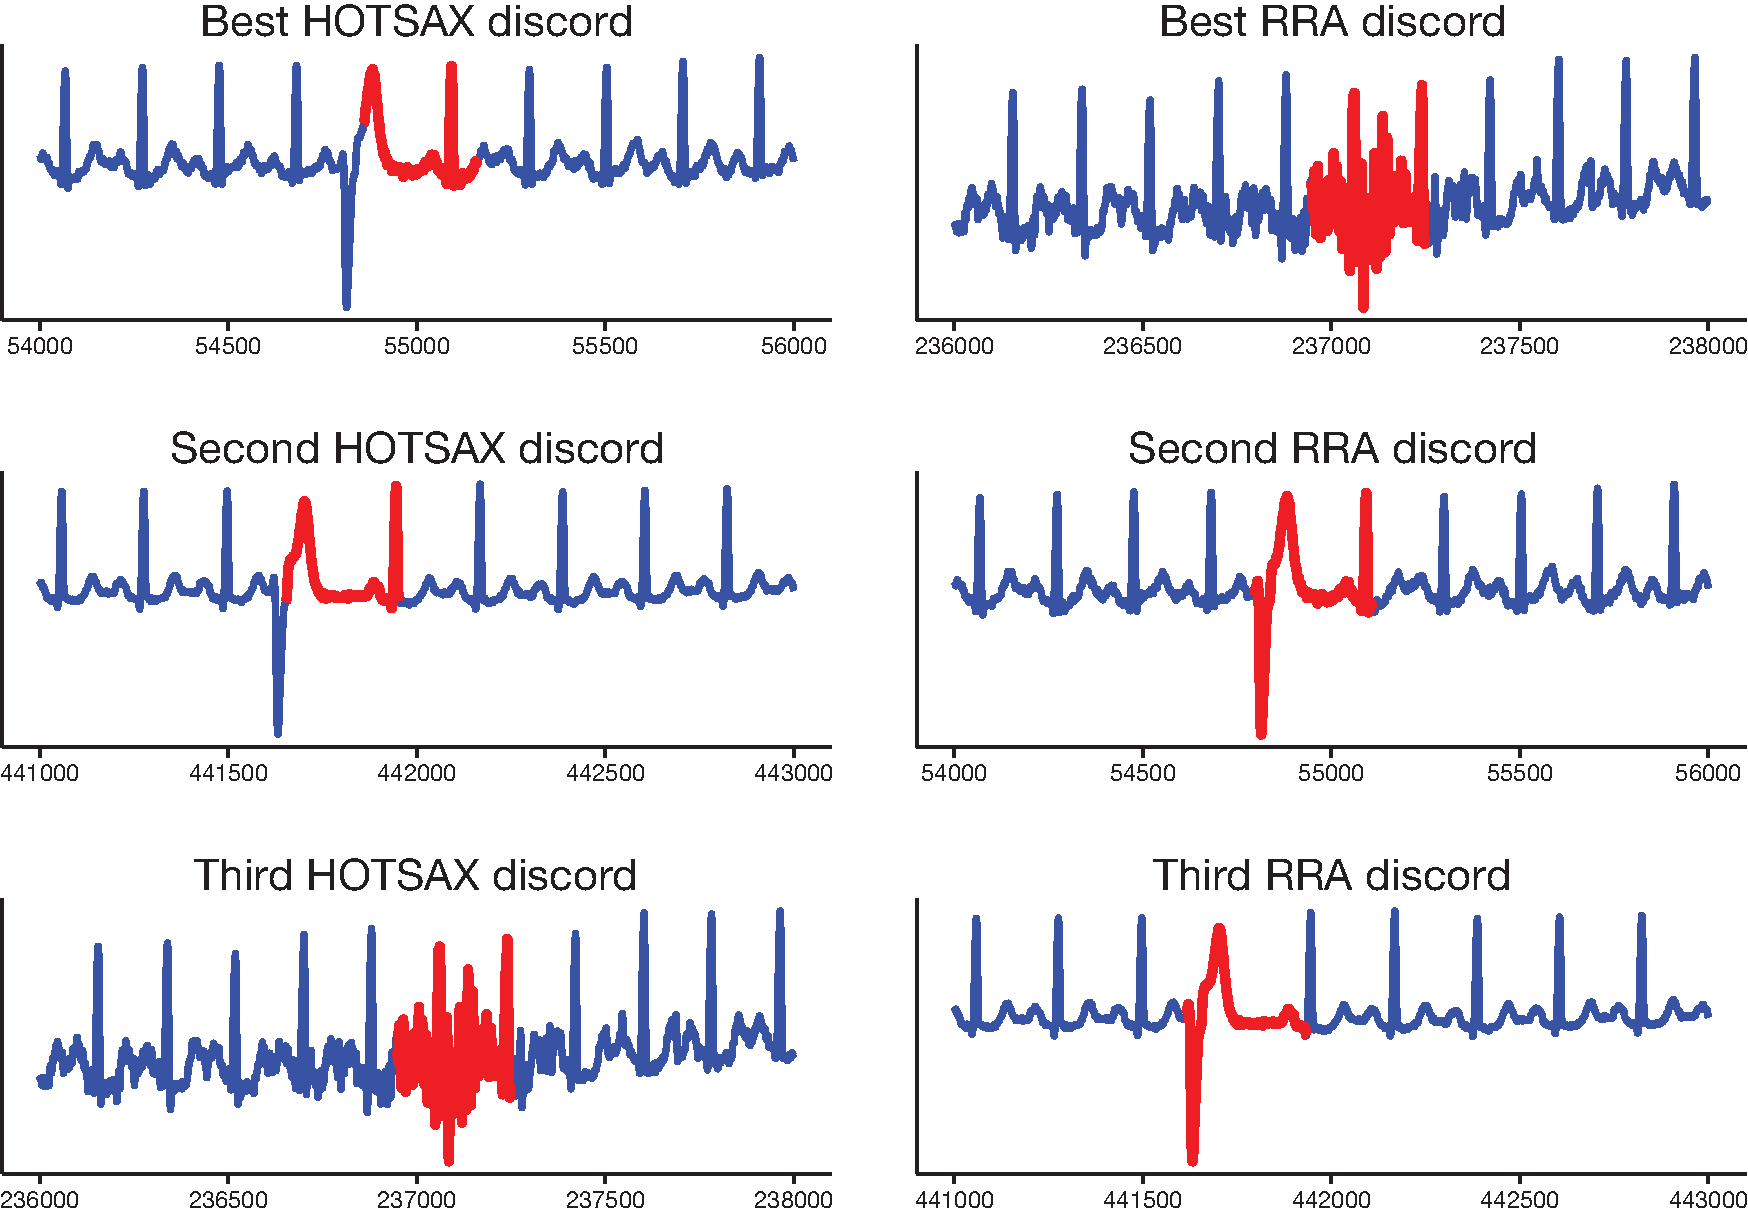
\includegraphics[width=84mm]{ECG300.pdf}
   \caption{The comparison of discords ranking by HOTSAX and RRA algorithms from ECG300 dataset of length 536'976. RRA ranked the shorter discord first due to the larger value of normalized by the subsequence length Euclidean distance (Eq.\eqref{dist}) to its nearest non-self match: the best discord has length 302, whereas the second and third discords have a length of 312 and 317 respectively.}
   \label{fig:ecg300}
\end{figure}

We compared the algorithms performance in terms of calls to the distance computation routine, which, as pointed out in \cite{hot_sax}, typically accounts for up to 99\% of these algorithms' computation time. Table \ref{perf_table} compares the number of distance function calls made by the competing techniques. Note that in the ECG300 dataset (which is record 300 of the MIT-BIH ST change database \cite{physionet}), RRA failed to rank discords in the same order as the HOTSAX algorithm. 

Our rule density-based algorithm was also able to discover anomalies in \textbf{all} data sets, though more careful parameter selection was needed at times; nevertheless, we found that this technique allows the discovery of very short anomalies which other evaluated techniques missed. For example, in the spatial trajectory dataset, the rule density-based technique was the only method capable of discovering a short, true anomaly that was intentionally planted by taking a detour.

\begin{figure}[t]
   \centering
   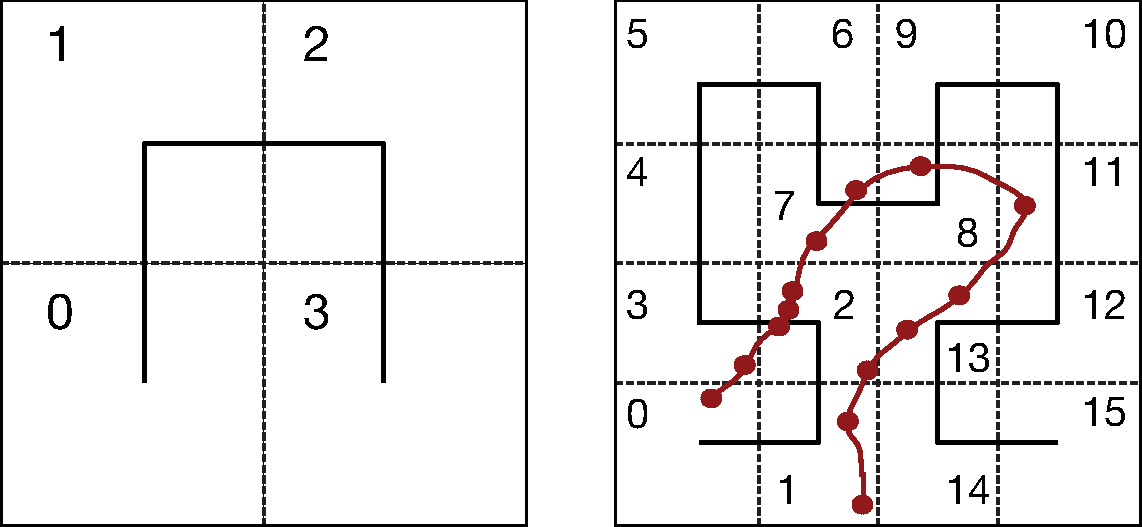
\includegraphics[width=80mm]{hilbert.pdf}
   \caption{Approximations of the Hilbert space filling curve (first order at the left, second order at the right panel) and a trajectory conversion example. The trajectory shown at the right panel is converted into the sequence \{0,3,2,2,2,7,7,8,11,13,13,2,1,1\} by converting each recorded spatial position into the enclosing Hilbert cell id.}   
   \label{fig:hilbert}
\end{figure}

To summarize, the rule density-based approach, when used alone, is extremely fast, but it has difficulty discriminating and ranking subtle discords. Incorporating the grammatical context into the distance-based RRA algorithm, however, enables the efficient discovery of discords in all data sets. RRA is much faster than HOTSAX and brute force, and it allows for the discovery of variable-length discords. 

%\begin{figure}[t]
   %\centering
   %\includegraphics[width=76mm]{hilbert.eps}
   %\caption{Approximations of the Hilbert space filling curve (first order at the left, second order at the right panel) and a trajectory conversion example. The trajectory shown at the right panel is converted into the sequence \{0,3,2,2,2,7,7,8,11,13,13,2,1,1\} by converting each recorded spatial position into the enclosing Hilbert cell id.}   
   %\label{fig:hilbert}
%\end{figure}

\begin{figure}[t]
   \centering
   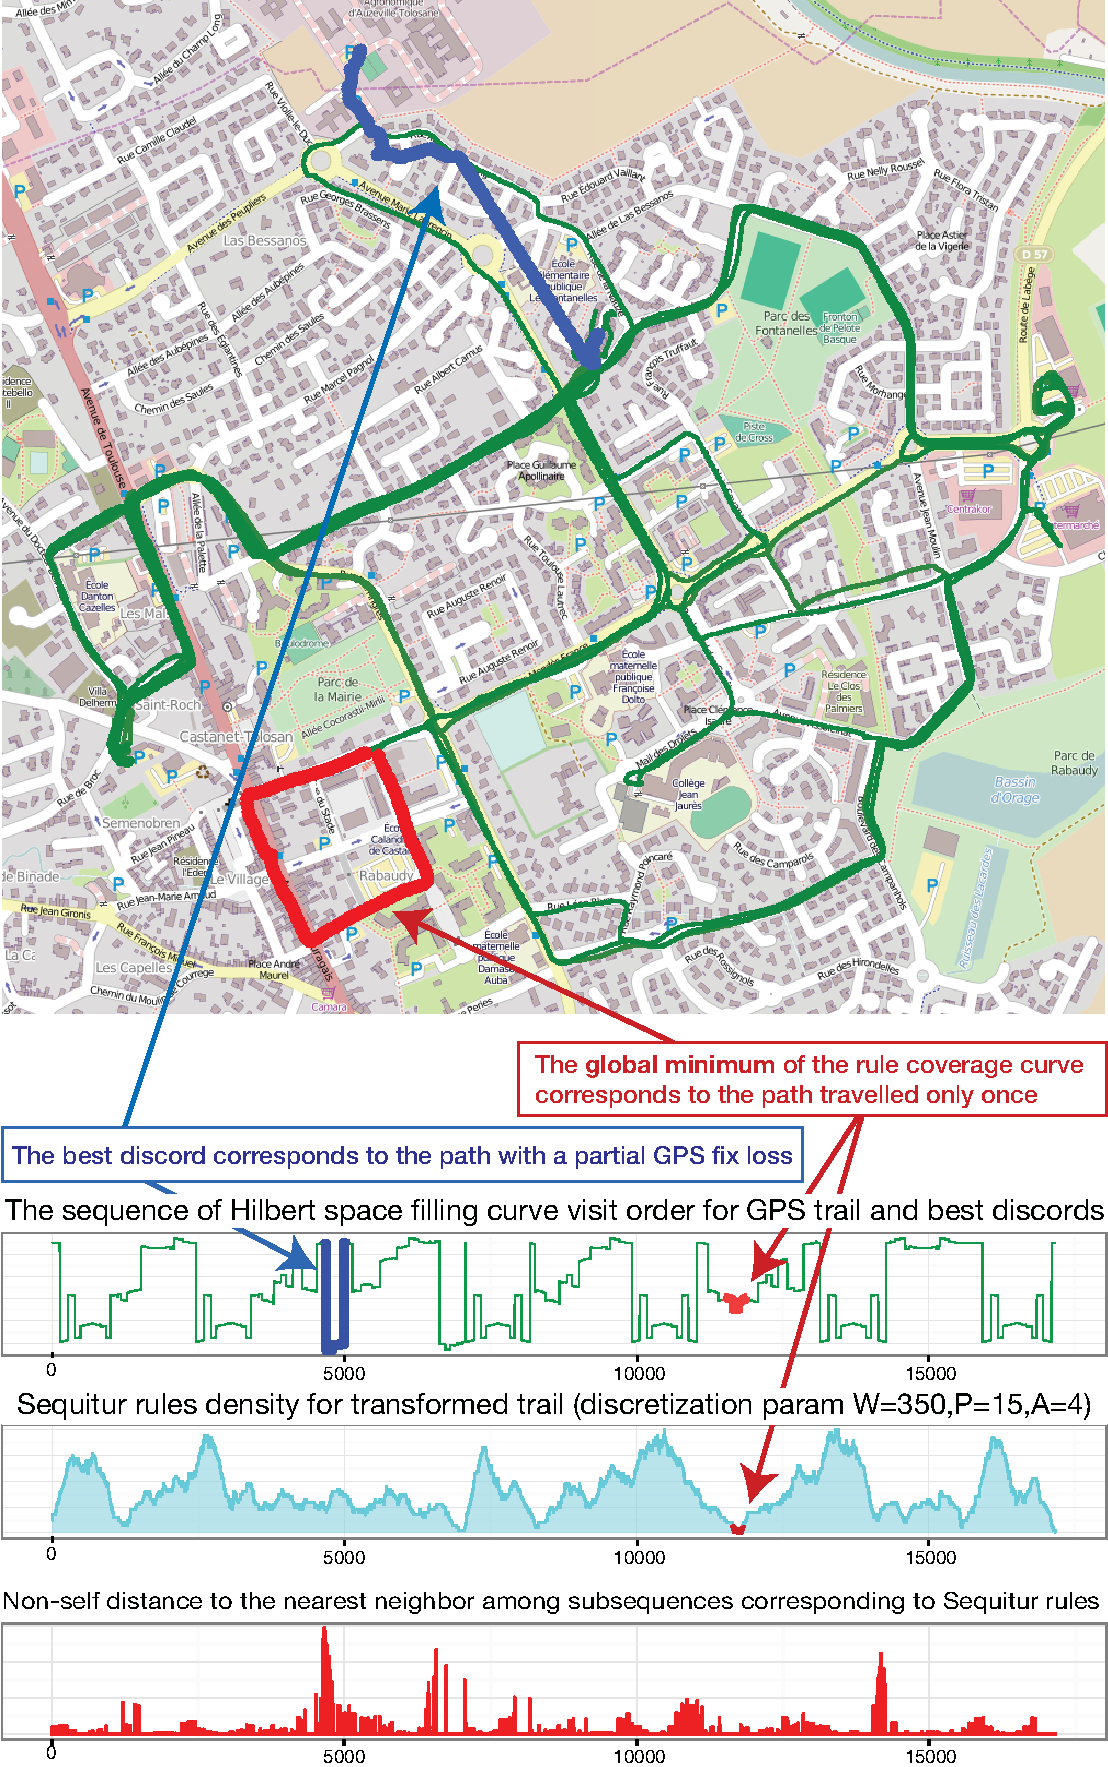
\includegraphics[width=82mm]{path_figure-option-new.pdf}
   \caption{An example of anomaly discovery in the Hilbert SFC transformed GPS track. The true anomaly, corresponding to the unique detour, was discovered by the rule density curve global minima, which reaches 0 at the interval of length 9, the best RRA discord of length 366 corresponds to the path traveled with a partial GPS fix (abnormal path running across properties). Note that RRA approach was not able to capture the anomalous detour.}   
   \label{fig:gps}
\end{figure}

\subsection{Spatial trajectory case study}
To demonstrate the utility of our technique for discovering anomalies of an \textit{unknown nature}, we performed a case study on spatial trajectory data. The trajectory data is intrinsically complex to explore for regularity since patterns of movement are often driven by unperceived goals and constrained by unknown environmental settings. 

The data used in this study was gathered from a GPS device which recorded location coordinates and times while commuting during a typical week by car and bicycle. 

To apply RRA to the trajectory, the multi-dimensional trajectory data (time, latitude, longitude) was transformed into a sequence of scalars. To achieve this, the trajectory points were mapped to the visit order of a Hilbert space filling curve (SFC) \cite{hilbert} embedded in the trajectory manifold space and indexed by the recorded times in the visit order (Figure \ref{fig:hilbert}, right panel). The Hilbert SFC was chosen to reduce the distortion on the data's spatial locality. The Hilbert SFC-transformed trajectory produces a time series, which is then passed to the RRA algorithm for anomaly discovery.

\begin{figure}[!ht]   
   \centering
   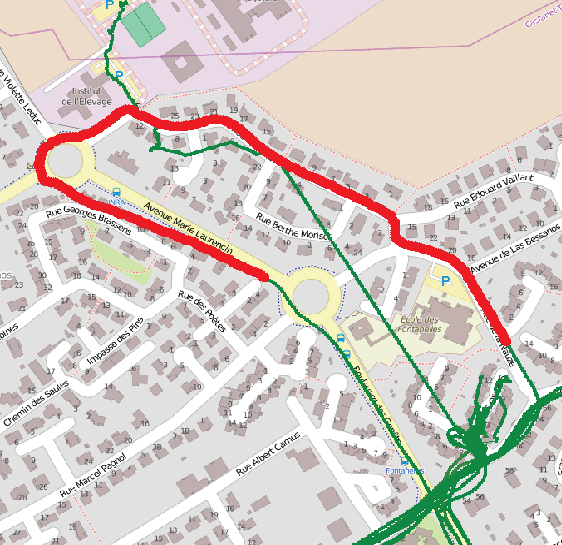
\includegraphics[width=84mm]{gps_zoom_0.pdf}
   \caption{The second discord discovered by the RRA algorithm highlights a uniquely traveled segment.}
   \label{fig:gps2}   
   \vspace{2em}
   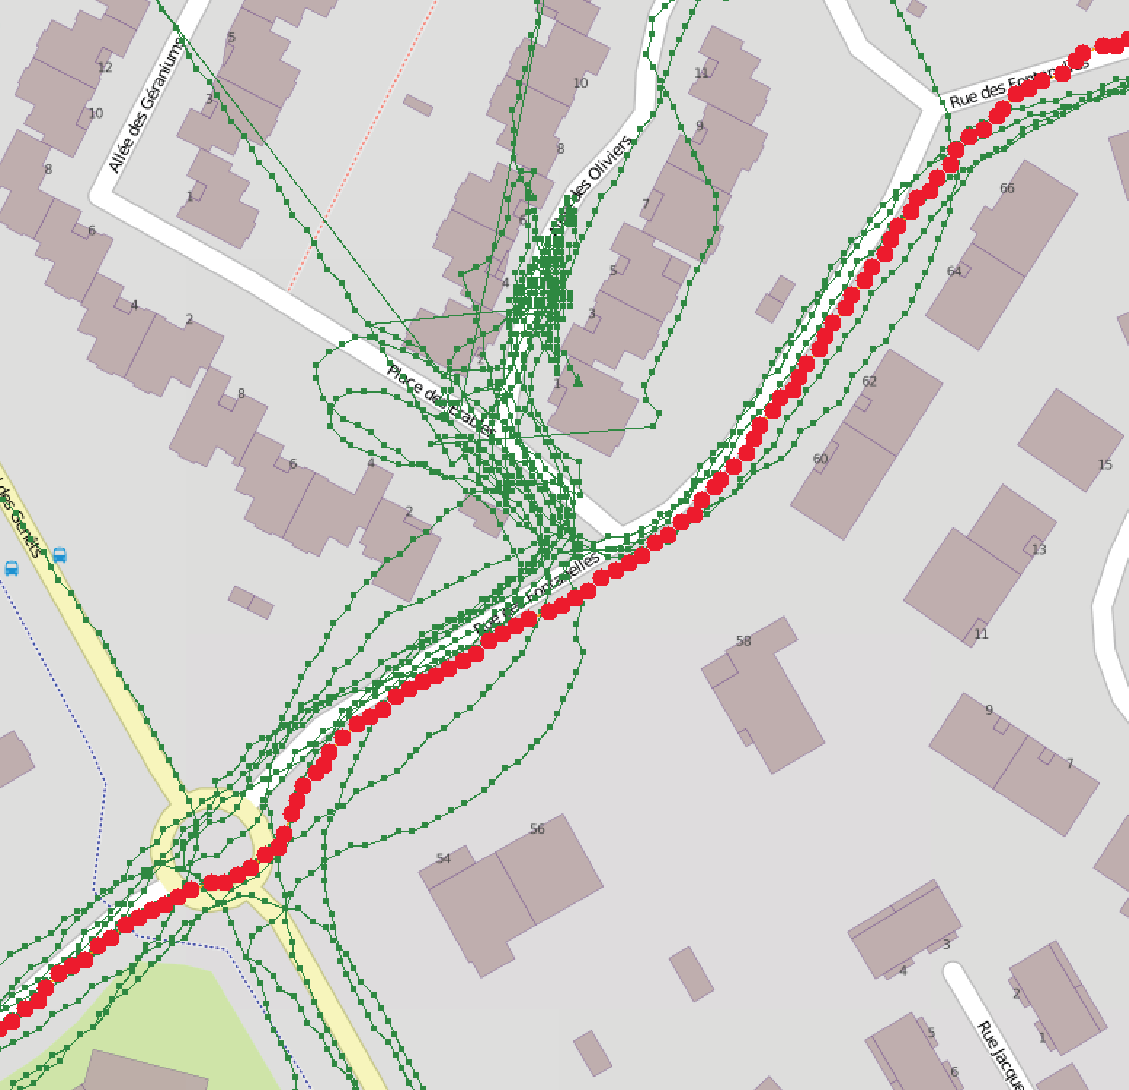
\includegraphics[width=84mm]{gps_zoom_1.pdf}
   \caption{The third discord discovered by the RRA algorithm highlights an abnormal behavior that does not conform to the usual pattern of exiting and entering the block's parking lot.}
   \label{fig:gps_zoom}
\end{figure}

To visualize this data transformation approach, consider Figure \ref{fig:hilbert} showing a Hilbert SFC of first order in the left panel and one of second order in the right panel. Note, that the left panel is divided into 4 quadrants and the first-order curve is drawn through their center points. The quadrants are ordered such that any two which are adjacent in the ordering share a common edge. In the next step, shown in the right panel, each of the quadrants of the left panel are divided into 4 more quadrants and, in all, 4 ``scaled-down'' first order curves are drawn and connected together. Note that the adjacency property of consecutive squares is maintained. As shown, maintaining adjacency helps to preserve spatial locality -- points close in space are generally close in their Hilbert values. For our trajectory experimentation, we have used a Hilbert SFC of order eight. 

In general, a trajectory anomaly is defined as a sub-trajec\-tory path that is atypical in the set of paths taken by an individual. Specifically, an anomaly can either be a sub-trajectory that occurs in rarely visited spatial regions such as a detour, or a novel path taken within a frequently visited spatial region. The second type of trajectory anomaly is important because it considers the order in which the various locations are visited. For instance, if multiple points in a space are visited frequently, the occurrence of a visit to these points is not an anomaly by itself; however, the occurrence of visiting these points in an unseen order is an anomaly. To evaluate the proposed algorithm's efficiency in these specific settings, we also intentionally planted an anomaly by taking an atypical route.

Figure \ref{fig:gps} shows the results of the discovered anomalies in the GPS track by both proposed algorithms. As shown, the rule density curve pinpoints an unusual detour deviating from a normal route significantly (red colored segment), the RRA algorithm highlighted a trajectory segment which was travelled with a partial GPS signal fix, but close to previously traveled routes (blue segment). This results highlight the difference in the algorithms' sensitivity due to their nature: the rule density curve-based approach finds algorithmically anomalous, short subsequences (shorter than the specified sliding window length) in the symbolic space of discretized values, whereas RRA is capable to rank algorithmically similar symbolic subsequences by discordance using their real representation.

While the second RRA-discovered discord shown in Figure \ref{fig:gps2} highlights a unique path, the third discord shown in Figure \ref{fig:gps_zoom} spotlights the algorithm's sensitivity and ability to capture subtle anomalies. The shown discord corresponds to an abnormal behavior within frequently traveled spatial regions -- not visiting the block's parking lot when traveling through the area. 

\subsection{Discretization parameters selection}
Similar to other discretization-based learning techniques, it is difficult to pinpoint a solution that offers the best trade-off between gain in tractability and loss in accuracy. Nevertheless, we found that within the grammar-based paradigm, the sliding window length parameter is not as critical as it is for most of the existing anomaly and motif detection algorithms, since it is just the "seed" size. Specifically, we found that the rule density curve facilitates the discovery of patterns that are much shorter than the window size, whereas the RRA algorithm naturally enables the discovery of longer patterns. Second, we observed that when the selection of discretization parameters is driven by the context, such as using the length of a heartbeat in ECG data, a weekly duration in power consumption data, or an observed phenomenon cycle length in telemetry, sensible results are usually produced. 

In addition, we found that the rule density approach alone is more sensitive to parameter choices than it is when incorporated into the RRA distance-based algorithm. Consider an example shown in Figure \ref{fig:area} where we used the ECG0606 dataset featuring a single true anomaly (the dataset overview is shown in Figure \ref{fig:ecg}). Since the discretization parameters affect both the precision of raw signal approximation and the size of the resulting grammar, by sampling this space and recording both algorithms' results we found that the area where the RRA algorithm discovered the true anomaly is twice as large as the same area for the rule density curve-based algorithm. In particular, when we varied the window size in the range $[10,500]$, PAA size in $[3,20]$, and the alphabet size in $[3,12]$; the rule density curve-based algorithm successfully discovered the anomaly for 1460 parameter combinations whereas RRA for 7100.

\begin{figure}[t]
   \centering
   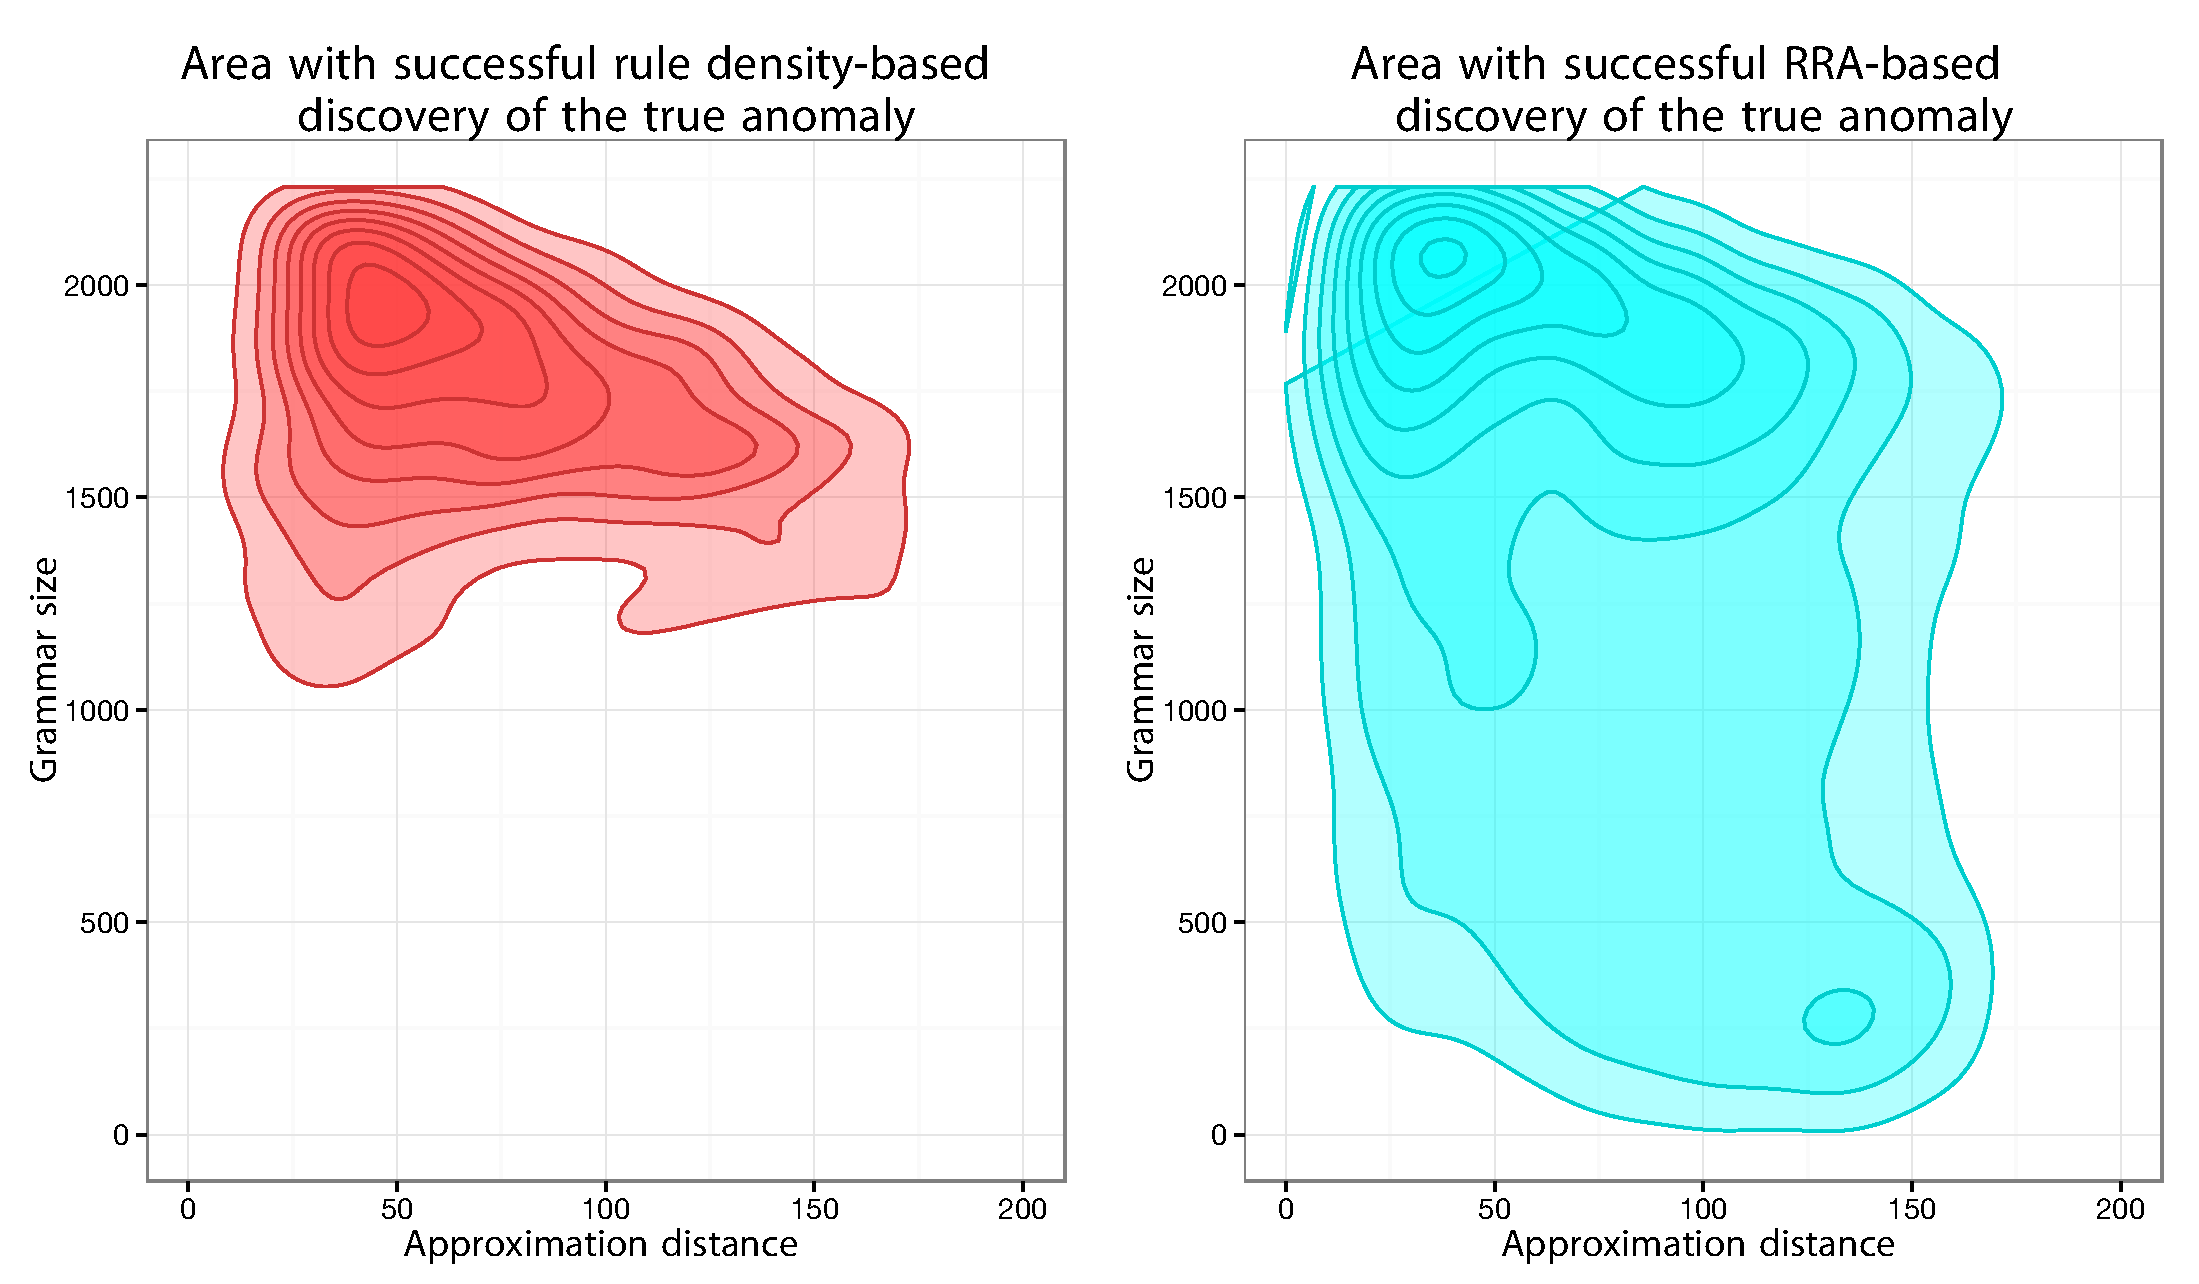
\includegraphics[width=84mm]{ecg0606_areas.pdf}
   \caption{An illustration from our exploratory study concerned with optimal parameters selection based on the constructed grammar properties. Both plots show boundaries of optimal parameter choices: left panel for the rule density curve-based algorithm, right panel for RRA. Note that RRA algorithm-corresponding area is much larger indicating its robustness.}
   \label{fig:area}
\end{figure}

\begin{figure*}[t]
   \centering
   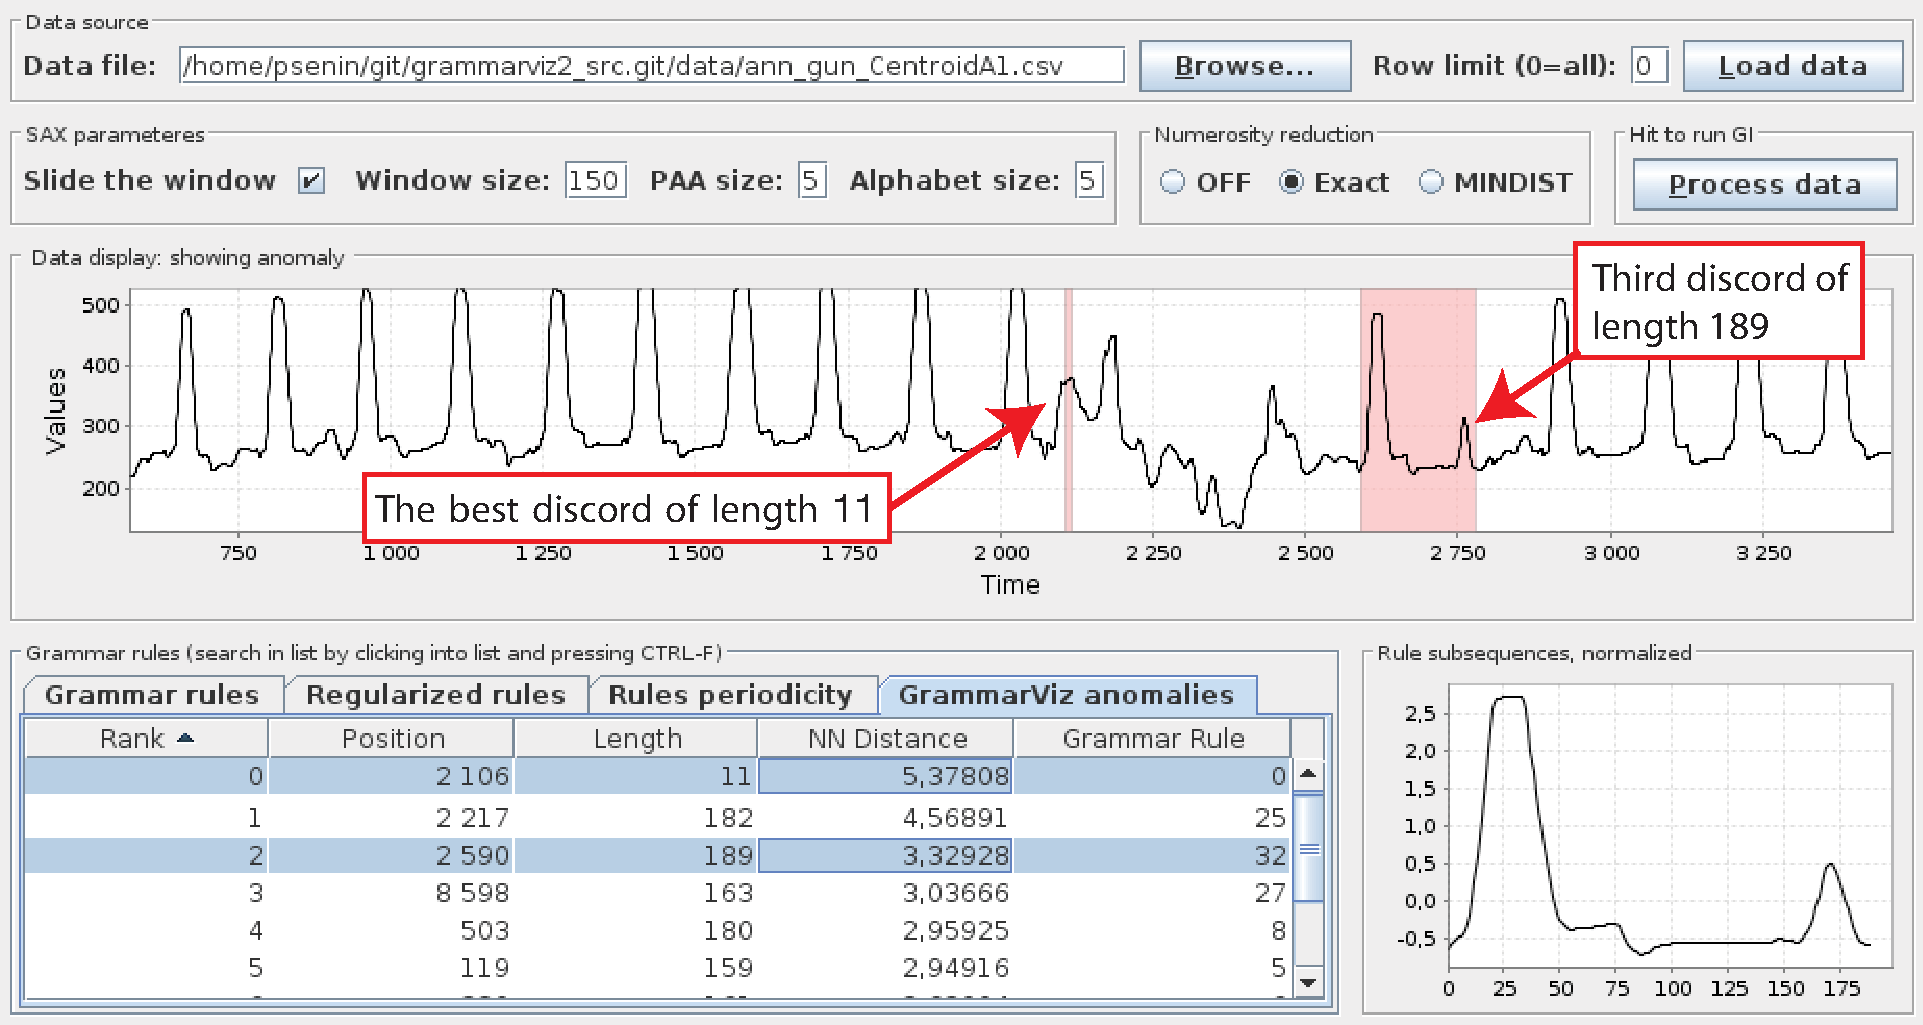
\includegraphics[width=\textwidth]{VideoData2.pdf}
   \caption{Incorporating the RRA algorithm in GrammarViz\,2.0 \cite{grammarviz2}. The screenshot shows its application to the recorded video data set \cite{param_free}. As shown, when configured with a window length of 150, RRA was able to detect multiple discords whose lengths vary from 11 to 189.}
   \label{fig:app2}
\end{figure*}

\subsection{Visualization}
As we pointed out before, to explore the properties of algorithmically anomalous subsequences, we have incorporated both algorithms proposed in this paper into our visualization tool called GrammarViz\,2.0 \cite{grammarviz2}. Figure \ref{fig:app2} shows the screenshot of GrammarViz\,2.0 using the RRA algorithm to find anomalies in a recorded video dataset. The discovered candidate anomalies are ranked by the distances to their nearest non-self matches. As shown in the ``Length" column, all candidate anomalies have different lengths. The highlighted subsequences in the upper panel correspond to the anomalies selected in the bottom panel.

Figure \ref{fig:app} shows the anomalies discovered in the same dataset using the rule density curve-based approach. As shown, we use the blue color intensity to express the grammar rules density: the darker is the shade, the higher is the corresponding value in rule density curve (i.e., the higher is rule count). Thus, the white-shaded regions denote the best potential anomalies since they correspond to global minima intervals in the rule density curve. 

Incorporating the proposed algorithms in our visualization tool allows interactive and efficient user-driven parameter tuning, as well as navigation and visualization of the results.

\begin{figure*}[t]
   \centering
   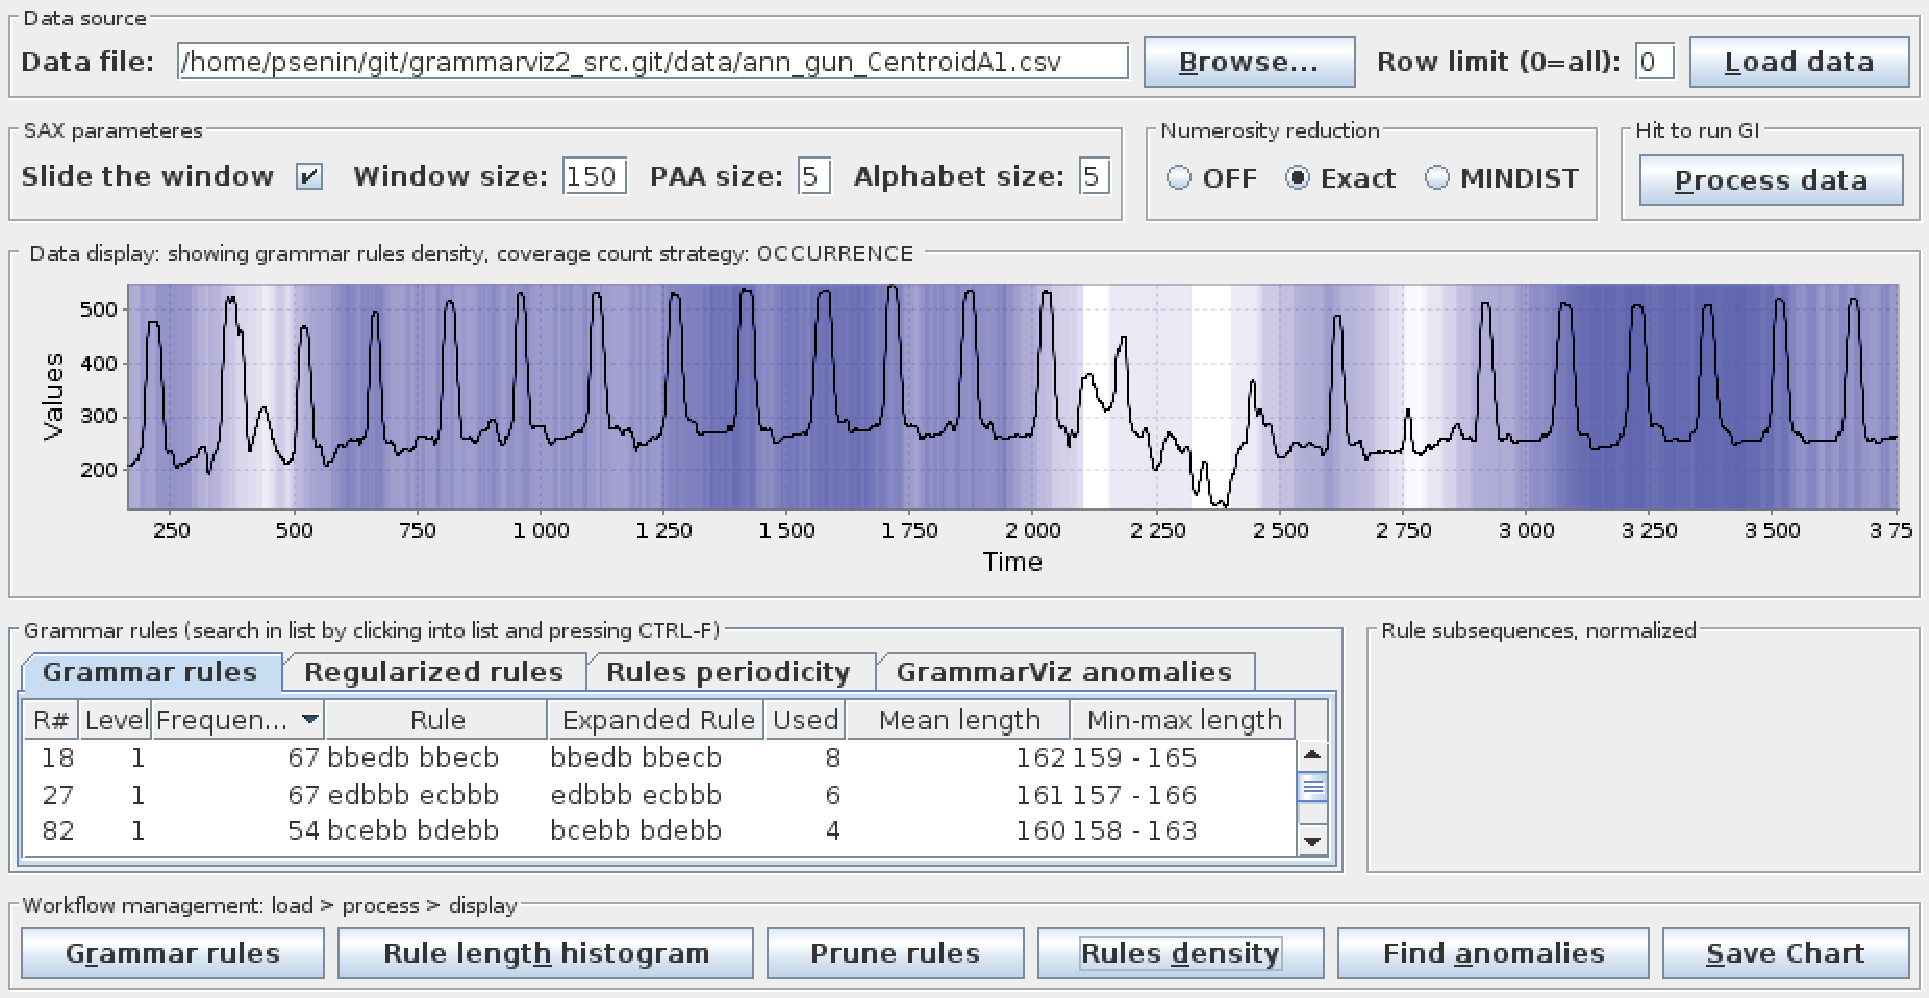
\includegraphics[width=\textwidth]{VideoData.pdf}
   \caption{Incorporating the rule-density-curve approach in GrammarViz\,2.0 \cite{grammarviz2}. The varying degrees of shades in the background correspond to \textit{rule density} curve values; the non-shaded (white) intervals pinpoint true anomalies.}
   \label{fig:app}
\end{figure*}

\section{Previous Work on Anomaly\\ Detection}
The brute force solution for the problem of time series anomaly detection or, more specifically, the discovery of a discord of a given length $n$ in time series $T$ of length $m$, needs to consider all possible distances between each subsequence $C$ of length $n$ and all of its non-self matches $M$ ($C,M \in T$). This method has $O(m^{2})$ complexity and is simply untenable for large data sets. 

To mitigate this heavy computational requirement, previous work suggests that the subsequence comparisons should be reordered for efficient pruning. For example HOTSAX \cite{hot_sax}, which is the pioneering work on discord discovery, suggests a fast heuristic technique that is capable of true discord discovery by reordering subsequences by their potential degree of discordance. Similarly in \cite{hashing}, the authors use locality sensitive hashing to estimate similarity between shapes with which they can efficiently reorder the search to discover unusual shapes. The authors of \cite{haar_1} and \cite{haar_2} use Haar wavelets and augmented tries to achieve effective pruning of the search space. While these approaches achieve a speed-up of several orders of magnitude over the brute-force algorithm, their common drawback is that they all need the length of a potential anomaly to be specified as the input, and they output discords of a fixed length. In addition, even with pruning, they rely on the distance computation which, as suggested by Keogh et al. \cite{hot_sax}, accounts for more than 99\% of these algorithms run-time.  

An interesting approach to find anomalies in a very large database (terabyte-sized data set) was shown by Yankov et al.~\cite{disk}. The authors proposed an algorithm that requires only two scans through the database. However, this method needs an anomaly defining range $r$ as the input. In addition, when used to detect an unusual subsequence within a time series, it also requires the length of the potential discord. 

Some techniques introduced approximate solutions that do not require distance computation on the raw time series. VizTree \cite{viztree} is a time series visualization tool that allows for the discovery of both frequent and rare (anomalous) patterns simultaneously. VizTree utilizes a trie (a tree-like data structure that allows for a constant time look-up) to decode the frequency of occurrences for all patterns in their discretized form. Similar to that defined in VizTree, Chen et al.\cite{ano_pattern} also consider anomalies to be the most infrequent time series patterns. The authors use support count to compute the anomaly score of each pattern. Although the definition of anomalies by Chen et al. is similar to discords, their technique requires more input parameters such as the precision of the slope $e$, the number of anomalous patterns $k$, or the minimum threshold. In addition, the anomalies discussed in their paper contain only two points. Wei et al. \cite{bitmaps} suggest another method that uses time series bitmaps to measure similarity. 

Finally, some previous work has examined the use of algorithmic randomness for time series anomaly discovery. Arning et al.~\cite{regex} proposed a linear time complexity algorithm for the sequential data anomaly detection problem from databases. Simulating a natural mechanism of memorizing previously seen data entities with regular-expression based abstractions capturing observed redundancy, their technique has been shown capable of detecting deviations in linear time. The proposed method relies on the user-defined entity size (the database record size). Alternatively, Keogh et al.~\cite{param_free} have shown an algorithmic randomness-based para\-meter-free approach to approximate anomaly detection (the WCAD algorithm). However, built upon use of an off-shelf compressor, their technique requires its numerous executions, which renders it computationally expensive; in addition, it requires the sliding window (i.e., anomaly) size to be specified.

\section{Conclusion and Future work}
In this work we hypothesized, that time series anomaly maps to algorithmically anomalous (i.e., incompressible with a grammatical inference algorithm) symbolic subsequence within the string obtained via time series symbolic discretization. The rationale behind this hypothesis is that if true, it allows for an efficient variable-length time series anomaly discovery approach.

Building upon subsequence discretization with SAX, which preserves the data structural context, and grammar induction with Sequitur, which guarantees discovery of all existing algorithmically-effective correlations by maintaining its invariants of uniqueness and utility at all times, we designed a generic framework for learning algorithmic regularities and detecting irregularities in time series in order to test our hypothesis. 

Using the framework, we constructed two time series anomaly discovery algorithms to empirically evaluate the hypothesis. One of these algorithms operates in the space of discretized data, whose dimensionality is typically much smaller than the original time series, and therefore is highly efficient. The output of this algorithm, namely the \textit{rule density curve}, was found to behave according to our hypothesis and provides an intuitive and efficient way for putative anomaly detection. Our second algorithm is based on the explicit distance computation and is capable to detect even subtle \textit{variable-length discords}.

Through an experimental evaluation, we have validated our hypothesis and have shown, that the proposed techniques are orders of magnitude more efficient than current state of the art without a loss in accuracy (Table \ref{perf_table}).

Since the grammar-based time series decomposition allows us to quantitatively assess the time series context through analysis of the grammar's hierarchical structure, the primary direction of our future effort is to analyze the effect of the discretization parameters on the algorithm's ability to discover contextually meaningful patterns. Since both techniques underlying our approach, namely, SAX discretization and grammatical inference with Sequitur, process the input time series from left to right, yet another research direction that suggests itself is the possibility of early anomaly detection in real-time data streams.

\section{Acknowledgments}
This research is partially supported by the National Science Foundation under Grant No. 1218325 and 1218318.

\begin{thebibliography}{99}
\vspace{1em}
%A
\bibitem{regex} 
Arning, A., Agrawal, R., \& Raghavan, P.,
{\em A Linear Method for Deviation Detection in Large Databases,}
In KDD (pp. 164-169) (1996)

%B
\bibitem{haar_2} 
Bu, Y., Leung, O., Fu, A., Keogh, E., Pei, J., Meshkin, S.,
{\em WAT: Finding Top-K Discords in Time Series Database},
In Proc. of SIAM Intl. Conf. on Data Mining (2007)

%C
\bibitem{chan_anomaly} 
Chandola, V., Cheboli, D., and Kumar, V.,
{\em Detecting Anomalies in a Time Series Database},
CS TR 09--004 (2009)

%C
\bibitem{ano_pattern} 
Chen, X., Zhan, Y.,
{\em Multi-scale Anomaly Detection Algorithm based on Infrequent Pattern of Time Series},
J. of Computational and Applied Mathematics (2008)

%C
\bibitem{ncd}
Cilibrasi, R., Vit{\'a}nyi, P.M.B.,
{\em Clustering by compression}, 
IEEE Trans. Inform. Theory (2005)

%F
\bibitem {grigorieff}
Ferbus-Zanda, M., Grigorieff, S.,
{\em Is Randomness ``Native'' to Computer Science?},
arXiv (2008)

%F
\bibitem{haar_1} 
Fu, A., Leung, O., Keogh, E., Lin, J.,
{\em Finding Time Series Discords based on Haar Transform},
In Proc. of Intl. Conf. on Adv. Data Mining and Applications (2006)

%G
\bibitem {physionet}
Goldberger, A.L. et al., 
{\em PhysioBank, PhysioToolkit, and PhysioNet: components of a new research resource for complex physiologic signals},
Circulation, 101(23) (2000)

%G
\bibitem{mdl}
Gr{\"u}nwald, P. D.,
{\em The Minimum Description Length Principle},
MIT Press (2007)

%G
\bibitem {outliers_survey}
Gupta, M., Gao, J., Aggarwal, C.C., Han, J.,
{\em Outlier Detection for Temporal Data: A Survey},
IEEE Trans. on Knowledge and Data Engineering, 25, 1 (2013)

%H
\bibitem{hawkins} 
Hawkins, D. M.,
{\em Identification of Outliers},
Chapman and Hall (1980)

%H
\bibitem {hilbert}
Hilbert, D.,
{\em \"{U}eber stetige Abbildung einer Linie auf ein Fl\"{a}chenst\"{u}ck}, 
Mathematische Annalen, 38:459--460 (1891)

%K
\bibitem {hot_sax}
Keogh, E., Lin, J., Fu, A.,
{\em HOT SAX: Efficiently Finding the Most Unusual Time Series Subsequence},
In Proc. ICDM'05 (2005)

%K
\bibitem {param_free}
Keogh, E., Lonardi, S., Ratanamahatana, C.A.,
{\em Towards parameter-free data mining},
In Proc. KDD (2004)

%K
\bibitem {kolmogorov}
Kolmogorov, A.N.,
{\em Three approaches to the quantitative definition of information},
Problems Inform. Transms. (1965)

%L
\bibitem {grammarviz}
Li, Y., Lin, J., and Oates, T.,
{\em Visualizing variable-length time series motifs},
In Proc. of SDM (2012)

%L
\bibitem {li_vitanyi}
Li, M. and Vit{\'a}nyi, P.M.B.,
{\em An Introduction to Kolmogorov Complexity and Its Applications},
Springer-Verlag (1993)

%L
\bibitem{viztree}
Lin, J., Keogh, E., Lonardi, S., Lankford, J.P., Nystrom, D. M.,
{\em Visually mining and monitoring massive time series},
In Proc. ACM SIGKDD Intn`l Conf. on KDD (2004)

%L
\bibitem {lin_motifs}
Lin, J., Keogh, E., Patel, P., and Lonardi, S.,
{\em Finding Motifs in Time Series},
The 2nd Workshop on Temporal Data Mining, the 8th ACM Int'l Conference on KDD (2002)

%M
\bibitem {per_lof}
Martin-L\"{o}f, Per,
{\em On the definition of random sequences},
Information and Control, MIT, 9:602-61 (1966)

%N
\bibitem{compression}
Nevill-Manning, C. and Witten, I.,
{\em Linear-Time, Incremental Hierarchy Inference for Compression},
In Proc. of IEEE Conference on Data Compression (1997)

%N
\bibitem {sequitur}
Nevill-Manning, C. and Witten, I.,
{\em Identifying Hierarchical Structure in Sequences: A linear-time algorithm},
Journal of Artificial Intelligence Research, 7, 67-84 (1997)

%O
\bibitem {msequitur}
Oates, T., Boedihardjo, A., Lin, J., Chen, C., Frankenstein, S., Gandhi, S.,
{\em Motif discovery in spatial trajectories using grammar inference},
In Proc. of ACM CIKM (2013)

%P
\bibitem{grammarviz_src}
Paper authors. Supporting webpage:
\url{http://github.com/GrammarViz2} (2015)

%P
\bibitem {sax}
Patel, P., Keogh, E., Lin, J., Lonardi, S.,
{\em Mining Motifs in Massive Time Series Databases},
In Proc. ICDM (2002)

%S
\bibitem {grammarviz2}
Senin, P., Lin, J., Wang, X., Oates, T., Gandhi, S., Boedihardjo, A.P., Chen, C., Frankenstein, S., Lerner, M.,
{\em GrammarViz 2.0: a tool for grammar-based pattern discovery in time series},
In Proc. ECML/PKDD (2014)

%S
\bibitem {solomonoff}
Solomonoff, R.J.,
{\em A formal theory of inductive inference. Part I},
Rockford Research Institute, Inc. (1962)

%V
\bibitem {dutchpd}
Van Wijk, J.J. and Van Selow, E.R., 
{\em Cluster and calendar based visualization of time series data},
In Proc. IEEE Symposium on Information Visualization (1999)

%W
\bibitem {hashing} 
Wei, L., Keogh, E., Xi, X.,
{\em SAXually explicit images: Finding unusual shapes},
In Proc. ICDM (2006)

%W
\bibitem{bitmaps} 
Wei, L., Kumar, N., Lolla, V., Keogh, E., Lonardi, S., Ratanamahatana, C.,
{\em Assumption-free Anomaly Detection in Time Series},
In Proc. SSDBM (2005)

%Y
\bibitem{disk}
Yankov, D., Keogh, E., Rebbapragada, U.,
{\em Disk aware discord discovery: finding unusual time series in terabyte sized data sets},
Knowledge and Information Systems, 241-262 (2008)

\end{thebibliography}
%\balancecolumns 

\end{document}
